% Options for packages loaded elsewhere
\PassOptionsToPackage{unicode}{hyperref}
\PassOptionsToPackage{hyphens}{url}
\PassOptionsToPackage{dvipsnames,svgnames,x11names}{xcolor}
%
\documentclass[
  letterpaper,
  DIV=11,
  numbers=noendperiod]{scrreprt}

\usepackage{amsmath,amssymb}
\usepackage{iftex}
\ifPDFTeX
  \usepackage[T1]{fontenc}
  \usepackage[utf8]{inputenc}
  \usepackage{textcomp} % provide euro and other symbols
\else % if luatex or xetex
  \usepackage{unicode-math}
  \defaultfontfeatures{Scale=MatchLowercase}
  \defaultfontfeatures[\rmfamily]{Ligatures=TeX,Scale=1}
\fi
\usepackage{lmodern}
\ifPDFTeX\else  
    % xetex/luatex font selection
\fi
% Use upquote if available, for straight quotes in verbatim environments
\IfFileExists{upquote.sty}{\usepackage{upquote}}{}
\IfFileExists{microtype.sty}{% use microtype if available
  \usepackage[]{microtype}
  \UseMicrotypeSet[protrusion]{basicmath} % disable protrusion for tt fonts
}{}
\makeatletter
\@ifundefined{KOMAClassName}{% if non-KOMA class
  \IfFileExists{parskip.sty}{%
    \usepackage{parskip}
  }{% else
    \setlength{\parindent}{0pt}
    \setlength{\parskip}{6pt plus 2pt minus 1pt}}
}{% if KOMA class
  \KOMAoptions{parskip=half}}
\makeatother
\usepackage{xcolor}
\setlength{\emergencystretch}{3em} % prevent overfull lines
\setcounter{secnumdepth}{5}
% Make \paragraph and \subparagraph free-standing
\makeatletter
\ifx\paragraph\undefined\else
  \let\oldparagraph\paragraph
  \renewcommand{\paragraph}{
    \@ifstar
      \xxxParagraphStar
      \xxxParagraphNoStar
  }
  \newcommand{\xxxParagraphStar}[1]{\oldparagraph*{#1}\mbox{}}
  \newcommand{\xxxParagraphNoStar}[1]{\oldparagraph{#1}\mbox{}}
\fi
\ifx\subparagraph\undefined\else
  \let\oldsubparagraph\subparagraph
  \renewcommand{\subparagraph}{
    \@ifstar
      \xxxSubParagraphStar
      \xxxSubParagraphNoStar
  }
  \newcommand{\xxxSubParagraphStar}[1]{\oldsubparagraph*{#1}\mbox{}}
  \newcommand{\xxxSubParagraphNoStar}[1]{\oldsubparagraph{#1}\mbox{}}
\fi
\makeatother

\usepackage{color}
\usepackage{fancyvrb}
\newcommand{\VerbBar}{|}
\newcommand{\VERB}{\Verb[commandchars=\\\{\}]}
\DefineVerbatimEnvironment{Highlighting}{Verbatim}{commandchars=\\\{\}}
% Add ',fontsize=\small' for more characters per line
\usepackage{framed}
\definecolor{shadecolor}{RGB}{241,243,245}
\newenvironment{Shaded}{\begin{snugshade}}{\end{snugshade}}
\newcommand{\AlertTok}[1]{\textcolor[rgb]{0.68,0.00,0.00}{#1}}
\newcommand{\AnnotationTok}[1]{\textcolor[rgb]{0.37,0.37,0.37}{#1}}
\newcommand{\AttributeTok}[1]{\textcolor[rgb]{0.40,0.45,0.13}{#1}}
\newcommand{\BaseNTok}[1]{\textcolor[rgb]{0.68,0.00,0.00}{#1}}
\newcommand{\BuiltInTok}[1]{\textcolor[rgb]{0.00,0.23,0.31}{#1}}
\newcommand{\CharTok}[1]{\textcolor[rgb]{0.13,0.47,0.30}{#1}}
\newcommand{\CommentTok}[1]{\textcolor[rgb]{0.37,0.37,0.37}{#1}}
\newcommand{\CommentVarTok}[1]{\textcolor[rgb]{0.37,0.37,0.37}{\textit{#1}}}
\newcommand{\ConstantTok}[1]{\textcolor[rgb]{0.56,0.35,0.01}{#1}}
\newcommand{\ControlFlowTok}[1]{\textcolor[rgb]{0.00,0.23,0.31}{\textbf{#1}}}
\newcommand{\DataTypeTok}[1]{\textcolor[rgb]{0.68,0.00,0.00}{#1}}
\newcommand{\DecValTok}[1]{\textcolor[rgb]{0.68,0.00,0.00}{#1}}
\newcommand{\DocumentationTok}[1]{\textcolor[rgb]{0.37,0.37,0.37}{\textit{#1}}}
\newcommand{\ErrorTok}[1]{\textcolor[rgb]{0.68,0.00,0.00}{#1}}
\newcommand{\ExtensionTok}[1]{\textcolor[rgb]{0.00,0.23,0.31}{#1}}
\newcommand{\FloatTok}[1]{\textcolor[rgb]{0.68,0.00,0.00}{#1}}
\newcommand{\FunctionTok}[1]{\textcolor[rgb]{0.28,0.35,0.67}{#1}}
\newcommand{\ImportTok}[1]{\textcolor[rgb]{0.00,0.46,0.62}{#1}}
\newcommand{\InformationTok}[1]{\textcolor[rgb]{0.37,0.37,0.37}{#1}}
\newcommand{\KeywordTok}[1]{\textcolor[rgb]{0.00,0.23,0.31}{\textbf{#1}}}
\newcommand{\NormalTok}[1]{\textcolor[rgb]{0.00,0.23,0.31}{#1}}
\newcommand{\OperatorTok}[1]{\textcolor[rgb]{0.37,0.37,0.37}{#1}}
\newcommand{\OtherTok}[1]{\textcolor[rgb]{0.00,0.23,0.31}{#1}}
\newcommand{\PreprocessorTok}[1]{\textcolor[rgb]{0.68,0.00,0.00}{#1}}
\newcommand{\RegionMarkerTok}[1]{\textcolor[rgb]{0.00,0.23,0.31}{#1}}
\newcommand{\SpecialCharTok}[1]{\textcolor[rgb]{0.37,0.37,0.37}{#1}}
\newcommand{\SpecialStringTok}[1]{\textcolor[rgb]{0.13,0.47,0.30}{#1}}
\newcommand{\StringTok}[1]{\textcolor[rgb]{0.13,0.47,0.30}{#1}}
\newcommand{\VariableTok}[1]{\textcolor[rgb]{0.07,0.07,0.07}{#1}}
\newcommand{\VerbatimStringTok}[1]{\textcolor[rgb]{0.13,0.47,0.30}{#1}}
\newcommand{\WarningTok}[1]{\textcolor[rgb]{0.37,0.37,0.37}{\textit{#1}}}

\providecommand{\tightlist}{%
  \setlength{\itemsep}{0pt}\setlength{\parskip}{0pt}}\usepackage{longtable,booktabs,array}
\usepackage{calc} % for calculating minipage widths
% Correct order of tables after \paragraph or \subparagraph
\usepackage{etoolbox}
\makeatletter
\patchcmd\longtable{\par}{\if@noskipsec\mbox{}\fi\par}{}{}
\makeatother
% Allow footnotes in longtable head/foot
\IfFileExists{footnotehyper.sty}{\usepackage{footnotehyper}}{\usepackage{footnote}}
\makesavenoteenv{longtable}
\usepackage{graphicx}
\makeatletter
\newsavebox\pandoc@box
\newcommand*\pandocbounded[1]{% scales image to fit in text height/width
  \sbox\pandoc@box{#1}%
  \Gscale@div\@tempa{\textheight}{\dimexpr\ht\pandoc@box+\dp\pandoc@box\relax}%
  \Gscale@div\@tempb{\linewidth}{\wd\pandoc@box}%
  \ifdim\@tempb\p@<\@tempa\p@\let\@tempa\@tempb\fi% select the smaller of both
  \ifdim\@tempa\p@<\p@\scalebox{\@tempa}{\usebox\pandoc@box}%
  \else\usebox{\pandoc@box}%
  \fi%
}
% Set default figure placement to htbp
\def\fps@figure{htbp}
\makeatother
% definitions for citeproc citations
\NewDocumentCommand\citeproctext{}{}
\NewDocumentCommand\citeproc{mm}{%
  \begingroup\def\citeproctext{#2}\cite{#1}\endgroup}
\makeatletter
 % allow citations to break across lines
 \let\@cite@ofmt\@firstofone
 % avoid brackets around text for \cite:
 \def\@biblabel#1{}
 \def\@cite#1#2{{#1\if@tempswa , #2\fi}}
\makeatother
\newlength{\cslhangindent}
\setlength{\cslhangindent}{1.5em}
\newlength{\csllabelwidth}
\setlength{\csllabelwidth}{3em}
\newenvironment{CSLReferences}[2] % #1 hanging-indent, #2 entry-spacing
 {\begin{list}{}{%
  \setlength{\itemindent}{0pt}
  \setlength{\leftmargin}{0pt}
  \setlength{\parsep}{0pt}
  % turn on hanging indent if param 1 is 1
  \ifodd #1
   \setlength{\leftmargin}{\cslhangindent}
   \setlength{\itemindent}{-1\cslhangindent}
  \fi
  % set entry spacing
  \setlength{\itemsep}{#2\baselineskip}}}
 {\end{list}}
\usepackage{calc}
\newcommand{\CSLBlock}[1]{\hfill\break\parbox[t]{\linewidth}{\strut\ignorespaces#1\strut}}
\newcommand{\CSLLeftMargin}[1]{\parbox[t]{\csllabelwidth}{\strut#1\strut}}
\newcommand{\CSLRightInline}[1]{\parbox[t]{\linewidth - \csllabelwidth}{\strut#1\strut}}
\newcommand{\CSLIndent}[1]{\hspace{\cslhangindent}#1}

\usepackage{booktabs}
\usepackage{longtable}
\usepackage{array}
\usepackage{multirow}
\usepackage{wrapfig}
\usepackage{float}
\usepackage{colortbl}
\usepackage{pdflscape}
\usepackage{tabu}
\usepackage{threeparttable}
\usepackage{threeparttablex}
\usepackage[normalem]{ulem}
\usepackage{makecell}
\usepackage{xcolor}
\KOMAoption{captions}{tableheading}
\makeatletter
\@ifpackageloaded{tcolorbox}{}{\usepackage[skins,breakable]{tcolorbox}}
\@ifpackageloaded{fontawesome5}{}{\usepackage{fontawesome5}}
\definecolor{quarto-callout-color}{HTML}{909090}
\definecolor{quarto-callout-note-color}{HTML}{0758E5}
\definecolor{quarto-callout-important-color}{HTML}{CC1914}
\definecolor{quarto-callout-warning-color}{HTML}{EB9113}
\definecolor{quarto-callout-tip-color}{HTML}{00A047}
\definecolor{quarto-callout-caution-color}{HTML}{FC5300}
\definecolor{quarto-callout-color-frame}{HTML}{acacac}
\definecolor{quarto-callout-note-color-frame}{HTML}{4582ec}
\definecolor{quarto-callout-important-color-frame}{HTML}{d9534f}
\definecolor{quarto-callout-warning-color-frame}{HTML}{f0ad4e}
\definecolor{quarto-callout-tip-color-frame}{HTML}{02b875}
\definecolor{quarto-callout-caution-color-frame}{HTML}{fd7e14}
\makeatother
\makeatletter
\@ifpackageloaded{bookmark}{}{\usepackage{bookmark}}
\makeatother
\makeatletter
\@ifpackageloaded{caption}{}{\usepackage{caption}}
\AtBeginDocument{%
\ifdefined\contentsname
  \renewcommand*\contentsname{Table of contents}
\else
  \newcommand\contentsname{Table of contents}
\fi
\ifdefined\listfigurename
  \renewcommand*\listfigurename{List of Figures}
\else
  \newcommand\listfigurename{List of Figures}
\fi
\ifdefined\listtablename
  \renewcommand*\listtablename{List of Tables}
\else
  \newcommand\listtablename{List of Tables}
\fi
\ifdefined\figurename
  \renewcommand*\figurename{Figure}
\else
  \newcommand\figurename{Figure}
\fi
\ifdefined\tablename
  \renewcommand*\tablename{Table}
\else
  \newcommand\tablename{Table}
\fi
}
\@ifpackageloaded{float}{}{\usepackage{float}}
\floatstyle{ruled}
\@ifundefined{c@chapter}{\newfloat{codelisting}{h}{lop}}{\newfloat{codelisting}{h}{lop}[chapter]}
\floatname{codelisting}{Listing}
\newcommand*\listoflistings{\listof{codelisting}{List of Listings}}
\makeatother
\makeatletter
\makeatother
\makeatletter
\@ifpackageloaded{caption}{}{\usepackage{caption}}
\@ifpackageloaded{subcaption}{}{\usepackage{subcaption}}
\makeatother

\usepackage{bookmark}

\IfFileExists{xurl.sty}{\usepackage{xurl}}{} % add URL line breaks if available
\urlstyle{same} % disable monospaced font for URLs
\hypersetup{
  pdftitle={Data and Visualization in R},
  pdfauthor={Alfredo Hernandez Sanchez, PhD},
  colorlinks=true,
  linkcolor={blue},
  filecolor={Maroon},
  citecolor={Blue},
  urlcolor={Blue},
  pdfcreator={LaTeX via pandoc}}


\title{Data and Visualization in R}
\usepackage{etoolbox}
\makeatletter
\providecommand{\subtitle}[1]{% add subtitle to \maketitle
  \apptocmd{\@title}{\par {\large #1 \par}}{}{}
}
\makeatother
\subtitle{A practical guide for social scientists}
\author{Alfredo Hernandez Sanchez, PhD}
\date{2026-05-07}

\begin{document}
\maketitle

\renewcommand*\contentsname{Table of contents}
{
\hypersetup{linkcolor=}
\setcounter{tocdepth}{2}
\tableofcontents
}

\bookmarksetup{startatroot}

\chapter*{Welcome}\label{welcome}
\addcontentsline{toc}{chapter}{Welcome}

\markboth{Welcome}{Welcome}

All tidy datasets are alike; each messy dataset set is messy in its own
way. If you have worked with data \emph{in the wild} you have surely
experienced the \textbf{frustration} of having to spend \textbf{more
time data cleaning than data analyzing}. The purpose of this book is to
accompany you throughout this unfortunate yet inevitable process and
offer some tricks and general guidelines that will make that journey
less strenuous. Back in the dark ages, before large language models
(LLMs) became part of our every day life, I taught a course on data
visualization at the Barcelona Institute of International Studies. This
book started as course notes with some code for students to tweak and
adapt to their needs. Today, memorizing the syntax of \texttt{R} code is
a far less marketable skill, and the fun part of data analysis and
visualization is ever more accessible. However, the grunt work of data
cleaning endures.

A special thanks goes out to the many students whose efforts, questions,
and feedback served as inspiration for this book!

\section*{Contact}\label{contact}
\addcontentsline{toc}{section}{Contact}

\markright{Contact}

This book is in open review. If you have any questions, comments or
suggestions; please report an issue on
\href{https://github.com/alfredo-hs/dviz_book}{GitHub}.

\section*{Build Information}\label{build-information}
\addcontentsline{toc}{section}{Build Information}

\markright{Build Information}

This book was built using R version 4.4.0 (2024-04-24). For specific
package versions please see the session information below:

\begin{verbatim}
R version 4.4.0 (2024-04-24)
Platform: aarch64-apple-darwin20
Running under: macOS Sonoma 14.2.1

Matrix products: default
BLAS:   /Library/Frameworks/R.framework/Versions/4.4-arm64/Resources/lib/libRblas.0.dylib 
LAPACK: /Library/Frameworks/R.framework/Versions/4.4-arm64/Resources/lib/libRlapack.dylib;  LAPACK version 3.12.0

locale:
[1] en_US.UTF-8/en_US.UTF-8/en_US.UTF-8/C/en_US.UTF-8/en_US.UTF-8

time zone: Europe/Vilnius
tzcode source: internal

attached base packages:
[1] stats     graphics  grDevices utils     datasets  methods   base     

loaded via a namespace (and not attached):
 [1] compiler_4.4.0    fastmap_1.2.0     cli_3.6.5         tools_4.4.0      
 [5] htmltools_0.5.8.1 rstudioapi_0.17.1 rmarkdown_2.29    knitr_1.50       
 [9] jsonlite_2.0.0    xfun_0.53         digest_0.6.37     rlang_1.1.7      
[13] evaluate_1.0.5   
\end{verbatim}

\section*{License}\label{license}
\addcontentsline{toc}{section}{License}

\markright{License}

{Data Visualization for Social Science} by {Alfredo Hernandez Sanchez}
is licensed under a Creative Commons
Attribution-NonCommercial-ShareAlike 4.0 International License.Based on
a work at https://github.com/alfredo-hs/dviz\_book.

\bookmarksetup{startatroot}

\chapter{Introduction}\label{introduction}

In an experiment conducted by researchers from University College London
(Mcmanus and Gesiak 2014), 277 participants were asked to look at
several pairs of paintings: one of the pairs was an original by abstract
painter Piet Mondrian, and the other was fake version that closely
resembled it.\footnote{The pseudo-Mondrians were created by jittering
  all the lines in the original but keeping the same relative positions.}
The participants where asked:

\begin{quote}
When looking at the pictures you should decide overall which you thinks
looks better, in that it looks nicer, it looks better organised, or it
looks better balanced.
\end{quote}

The results suggested that people could identify the originals with some
degree of accuracy (\(\mu\) 54.7\%, SE .40). This experiment ``implies
people know something about what makes a real Mondrian.'' In other
words, we have an \emph{intuition} of proportion and beauty.

\begin{Shaded}
\begin{Highlighting}[]
\FunctionTok{library}\NormalTok{(ggplot2)}
\FunctionTok{library}\NormalTok{(dplyr)}

\NormalTok{white }\OtherTok{=} \StringTok{"\#dde1e0"}
\NormalTok{blue }\OtherTok{=} \StringTok{"\#3450a2"}
\NormalTok{black }\OtherTok{=} \StringTok{"\#171916"}
\NormalTok{yellow }\OtherTok{=} \StringTok{"\#e7eb99"}
\NormalTok{orange }\OtherTok{=} \StringTok{"\#e4480a"}
\NormalTok{gray }\OtherTok{=} \StringTok{"\#2d2d2e"}

\FunctionTok{ggplot}\NormalTok{()}\SpecialCharTok{+}
  \FunctionTok{annotate}\NormalTok{(}\StringTok{"rect"}\NormalTok{, }\AttributeTok{xmin =} \DecValTok{0}\NormalTok{, }\AttributeTok{xmax =} \DecValTok{100}\NormalTok{, }\AttributeTok{ymin =} \DecValTok{0}\NormalTok{, }\AttributeTok{ymax =}\DecValTok{100}\NormalTok{, }\AttributeTok{fill=}\NormalTok{white, }\AttributeTok{alpha=}\NormalTok{.}\DecValTok{8}\NormalTok{)}\SpecialCharTok{+}
  \FunctionTok{annotate}\NormalTok{(}\StringTok{"rect"}\NormalTok{, }\AttributeTok{xmin =} \DecValTok{80}\NormalTok{, }\AttributeTok{xmax =} \DecValTok{100}\NormalTok{, }\AttributeTok{ymin =} \DecValTok{80}\NormalTok{, }\AttributeTok{ymax =} \DecValTok{100}\NormalTok{, }\AttributeTok{fill=}\NormalTok{gray)}\SpecialCharTok{+}
  \FunctionTok{annotate}\NormalTok{(}\StringTok{"rect"}\NormalTok{, }\AttributeTok{xmin =} \DecValTok{50}\NormalTok{, }\AttributeTok{xmax =} \DecValTok{80}\NormalTok{, }\AttributeTok{ymin =} \DecValTok{90}\NormalTok{, }\AttributeTok{ymax =} \DecValTok{100}\NormalTok{, }\AttributeTok{fill=}\NormalTok{yellow)}\SpecialCharTok{+}
  \FunctionTok{annotate}\NormalTok{(}\StringTok{"rect"}\NormalTok{, }\AttributeTok{xmin =} \DecValTok{80}\NormalTok{, }\AttributeTok{xmax =} \DecValTok{100}\NormalTok{, }\AttributeTok{ymin =} \DecValTok{0}\NormalTok{, }\AttributeTok{ymax =}\DecValTok{8}\NormalTok{, }\AttributeTok{fill=}\NormalTok{orange)}\SpecialCharTok{+}
  \FunctionTok{annotate}\NormalTok{(}\StringTok{"rect"}\NormalTok{, }\AttributeTok{xmin =} \DecValTok{0}\NormalTok{, }\AttributeTok{xmax =} \DecValTok{5}\NormalTok{, }\AttributeTok{ymin =} \DecValTok{20}\NormalTok{, }\AttributeTok{ymax =}\DecValTok{50}\NormalTok{, }\AttributeTok{fill=}\NormalTok{blue)}\SpecialCharTok{+}
  \FunctionTok{geom\_segment}\NormalTok{(}\FunctionTok{aes}\NormalTok{(}\AttributeTok{x=}\DecValTok{80}\NormalTok{, }\AttributeTok{y=}\DecValTok{100}\NormalTok{, }\AttributeTok{xend=}\DecValTok{80}\NormalTok{, }\AttributeTok{yend=}\DecValTok{2}\NormalTok{), }\AttributeTok{size=}\DecValTok{2}\NormalTok{, }\AttributeTok{color=}\NormalTok{black)}\SpecialCharTok{+}
  \FunctionTok{geom\_segment}\NormalTok{(}\FunctionTok{aes}\NormalTok{(}\AttributeTok{x=}\DecValTok{80}\NormalTok{, }\AttributeTok{y=}\DecValTok{90}\NormalTok{, }\AttributeTok{xend=}\DecValTok{2}\NormalTok{, }\AttributeTok{yend=}\DecValTok{90}\NormalTok{), }\AttributeTok{size=}\DecValTok{2}\NormalTok{, }\AttributeTok{color=}\NormalTok{black)}\SpecialCharTok{+}
  \FunctionTok{geom\_segment}\NormalTok{(}\FunctionTok{aes}\NormalTok{(}\AttributeTok{x=}\DecValTok{0}\NormalTok{, }\AttributeTok{y=}\DecValTok{50}\NormalTok{, }\AttributeTok{xend=}\DecValTok{5}\NormalTok{, }\AttributeTok{yend=}\DecValTok{50}\NormalTok{), }\AttributeTok{size=}\DecValTok{2}\NormalTok{, }\AttributeTok{color=}\NormalTok{black)}\SpecialCharTok{+}
  \FunctionTok{geom\_segment}\NormalTok{(}\FunctionTok{aes}\NormalTok{(}\AttributeTok{x=}\DecValTok{5}\NormalTok{, }\AttributeTok{y=}\DecValTok{90}\NormalTok{, }\AttributeTok{xend=}\DecValTok{5}\NormalTok{, }\AttributeTok{yend=}\DecValTok{20}\NormalTok{), }\AttributeTok{size=}\DecValTok{2}\NormalTok{, }\AttributeTok{color=}\NormalTok{black)}\SpecialCharTok{+}
  \FunctionTok{geom\_segment}\NormalTok{(}\FunctionTok{aes}\NormalTok{(}\AttributeTok{x=}\DecValTok{80}\NormalTok{, }\AttributeTok{y=}\DecValTok{20}\NormalTok{, }\AttributeTok{xend=}\DecValTok{2}\NormalTok{, }\AttributeTok{yend=}\DecValTok{20}\NormalTok{), }\AttributeTok{size=}\DecValTok{2}\NormalTok{, }\AttributeTok{color=}\NormalTok{black)}\SpecialCharTok{+}
  \FunctionTok{geom\_segment}\NormalTok{(}\FunctionTok{aes}\NormalTok{(}\AttributeTok{x=}\DecValTok{50}\NormalTok{, }\AttributeTok{y=}\DecValTok{90}\NormalTok{, }\AttributeTok{xend=}\DecValTok{50}\NormalTok{, }\AttributeTok{yend=}\DecValTok{98}\NormalTok{), }\AttributeTok{size=}\DecValTok{2}\NormalTok{, }\AttributeTok{color=}\NormalTok{black)}\SpecialCharTok{+}
  \FunctionTok{geom\_segment}\NormalTok{(}\FunctionTok{aes}\NormalTok{(}\AttributeTok{x=}\DecValTok{80}\NormalTok{, }\AttributeTok{y=}\DecValTok{80}\NormalTok{, }\AttributeTok{xend=}\DecValTok{100}\NormalTok{, }\AttributeTok{yend=}\DecValTok{80}\NormalTok{), }\AttributeTok{size=}\DecValTok{2}\NormalTok{, }\AttributeTok{color=}\NormalTok{black)}\SpecialCharTok{+}
  \FunctionTok{geom\_segment}\NormalTok{(}\FunctionTok{aes}\NormalTok{(}\AttributeTok{x=}\DecValTok{80}\NormalTok{, }\AttributeTok{y=}\DecValTok{8}\NormalTok{, }\AttributeTok{xend=}\DecValTok{99}\NormalTok{, }\AttributeTok{yend=}\DecValTok{8}\NormalTok{), }\AttributeTok{size=}\DecValTok{2}\NormalTok{, }\AttributeTok{color=}\NormalTok{black)}\SpecialCharTok{+}
  \FunctionTok{scale\_y\_continuous}\NormalTok{(}\AttributeTok{limits=}\FunctionTok{c}\NormalTok{(}\DecValTok{0}\NormalTok{,}\DecValTok{100}\NormalTok{), }\AttributeTok{expand =} \FunctionTok{c}\NormalTok{(.}\DecValTok{02}\NormalTok{,}\DecValTok{0}\NormalTok{))}\SpecialCharTok{+}
  \FunctionTok{scale\_x\_continuous}\NormalTok{(}\AttributeTok{limits=}\FunctionTok{c}\NormalTok{(}\DecValTok{0}\NormalTok{,}\DecValTok{100}\NormalTok{), }\AttributeTok{expand =} \FunctionTok{c}\NormalTok{(.}\DecValTok{02}\NormalTok{,}\DecValTok{0}\NormalTok{))}\SpecialCharTok{+}
  \FunctionTok{theme}\NormalTok{(}\AttributeTok{axis.title =} \FunctionTok{element\_text}\NormalTok{(}\AttributeTok{face =} \StringTok{"italic"}\NormalTok{, }\AttributeTok{size =} \DecValTok{20}\NormalTok{),}
        \AttributeTok{axis.text.x =} \FunctionTok{element\_blank}\NormalTok{(),}
        \AttributeTok{axis.text.y =} \FunctionTok{element\_blank}\NormalTok{(),}
        \AttributeTok{axis.ticks =} \FunctionTok{element\_blank}\NormalTok{(),}
        \AttributeTok{panel.background =} \FunctionTok{element\_blank}\NormalTok{(),}
        \AttributeTok{panel.grid =} \FunctionTok{element\_blank}\NormalTok{(),}
        \AttributeTok{panel.border =} \FunctionTok{element\_blank}\NormalTok{(),}
        \AttributeTok{axis.line =} \FunctionTok{element\_line}\NormalTok{())}
\end{Highlighting}
\end{Shaded}

\begin{figure}[H]

{\centering 
\includegraphics[width=0.8\linewidth,height=\textheight,keepaspectratio]{intro_files/figure-pdf/mondrian-fig-1.pdf}

}

\caption{An \emph{attempt} at a Mondrian using \texttt{ggplot2}}

\end{figure}%

One of the most fun things about data visualization is making things
that are beautiful. In making them, you learn a lot about not just the
patterns you are displaying, but the scope and limitations of the
underlying data. Having taught courses on data viz for several years, I
have found that there is a correlation between the effort put into
making a plot beautiful and how accurately it conveys the intended
message.

\section*{Why Visualize?}\label{why-visualize}
\addcontentsline{toc}{section}{Why Visualize?}

\markright{Why Visualize?}

Data visualization plays numerous roles in the social sciences, from
summarizing large amounts of information in a small space, to supporting
claims about patterns and relationships among a vast array of indicators
of human behavior.

Zinovyev (2010) identifies four types of visualizations in political
science:

\begin{quote}
\begin{itemize}
\tightlist
\item
  \emph{Statistical graphics and infographics} with extensive use of
  color, form, size, shape and style to superimpose many quantitative
  variables in the same chart or diagram
\item
  \emph{Geographical information systems (GIS)} to visualize
  geographically-linked data
\item
  \emph{Graph visualization or network maps} for representing relations
  between objects
\item
  Projection of multidimensional data on low-dimensional screens with
  further visualization, \emph{data cartography}
\end{itemize}
\end{quote}

In addition, visualization is often the last part of a data analysis
pipeline. To visualize a data set you must first answer some questions:

\begin{itemize}
\tightlist
\item
  What do I want to visualize?
\item
  Where can I get the data?
\item
  How should my data set look like?
\item
  What is the data telling me?
\end{itemize}

In other words, to create visualizations you must also know what data is
(or not) out there (literature review), develop an intuition about what
patterns you might find in it (research question/hypothesis), clean and
wrangle lots of often messy data sets (methodology), create the
visualization (results) and share it with your target audience
(discussion). Think of the process as writing a small research paper. A
single \texttt{.png} often speaks more than a thousand lines of code!

\subsection*{About this Book}\label{about-this-book}
\addcontentsline{toc}{subsection}{About this Book}

The examples used throughout this book are closely related to corruption
since that is one of my main areas of interest. This also allows me to
explore different types of data that social scientists are likely to
encounter such as surveys, text, networks, geo-locations, administrative
records (\emph{Big Data}), and regression models.

All used data is open source, though it often comes through
APIs\footnote{API is short for \emph{application programming interface}
  and it is a great way to get data directly from the source. Many data
  providers such as the World Bank offer APIs that connect directly to
  your R session.}. Sometimes, to access these data sets you need a
\emph{token} or \emph{secret}. For obvious reasons, I will not share my
own tokens here, but I will show you where the information you need
should go in the code. When possible, I will also provide a clean
version of the data used so you can experiment with it.

To keep things as simple as possible, the book follows this syntax:

\begin{itemize}
\tightlist
\item
  \texttt{packages} are placed inside a shaded box
  (e.g.~\texttt{ggplot2}),
\item
  common \texttt{functions()} are also inside a shaded box, and followed
  by parentheses (e.g.~\texttt{mutate()} from \texttt{tidyverse} or
  \texttt{class()} from base R),
\item
  less common \texttt{functions()} are the same, but the package is
  explicitly called \texttt{::} (e.g.~\texttt{reshape2::melt()}),
\item
  short R commands (e.g.~\texttt{\%in\%}), are also shaded, non-R
  commands are in bold (e.g.~\textbf{Ctrl + p}),
\item
  the common \emph{pipe} operator \texttt{\%\textgreater{}\%} will be
  used when possible in the code\footnote{For Windows users, the
    \texttt{\%\textgreater{}\%} shortcut in RStudio is \textbf{Ctrl +
    Shift + M} and for Mac users it is \textbf{Cmd + Shift + M}.} (i.e.,
  we will mostly use the \texttt{tidyverse} syntax over base R).
\end{itemize}

\subsection*{Recommended Readings}\label{recommended-readings}
\addcontentsline{toc}{subsection}{Recommended Readings}

This book does not expect a lot of familiarity with R or programming,
though some knowledge of statistics will be very helpful. The appendix
covers the basics of working with R and
\href{https://www.rstudio.com/products/rstudio/download/}{RStudio}
during the first few sessions. Some tutorial videos on the basics of
working with RStudio are available \href{}{here}. Similarly, you may
also consult the following open-source books on R:\footnote{For a
  comprehensive list of R-related books, consult the \emph{R-Project}
  \href{https://www.r-project.org/doc/bib/R-books.html}{Website}}

\begin{itemize}
\tightlist
\item
  \href{https://rc2e.com/}{\emph{R Cookbook}} (Long and Teetor 2019)
\item
  \href{https://r4ds.had.co.nz/}{\emph{R for Data Science}} (Grolemund
  and Wickham 2016)
\item
  \href{https://r-graphics.org/}{\emph{R Graphics Cookbook}} (Chang
  2018)
\item
  \href{https://csgillespie.github.io/efficientR/}{\emph{Efficient R
  Programming}} (Gillespie and Lovelace 2016)
\item
  \href{https://rstudio-education.github.io/hopr/}{\emph{Hands-on
  Programming with R}} (Grolemund 2014)
\item
  \href{https://clauswilke.com/dataviz/}{\emph{Fundamentals of Data
  Visualization}} (Wilke 2019)
\item
  \href{https://www.tidytextmining.com/}{\emph{Text Mining with R}}
  (Silge and Robinson 2017)
\item
  \href{https://cran.r-project.org/doc/manuals/R-intro.pdf}{\emph{An
  Introduction to R}} (Venables, Smith, and R Core Team 2021)
\item
  \href{https://bookdown.org/yihui/rmarkdown/}{\emph{R Markdown: The
  Definitive Guide}} (Xie, Allaire, and Grolemund 2018)
\item
  \href{https://bookdown.org/yihui/rmarkdown-cookbook/}{\emph{R Markdown
  Cookbook}} (Xie, Dervieux, and Riederer 2020)
\end{itemize}

\bookmarksetup{startatroot}

\chapter{The Grammar of Graphics}\label{ggbasics}

\section{\texorpdfstring{The \texttt{tidyverse}
packages}{The tidyverse packages}}\label{the-tidyverse-packages}

Throughout this course, we will be using tidy data principles\footnote{These
  principles are: a) each variable should have its own column, b) each
  observation should have its own row, and c) each value should have its
  own cell.} to create several types of visualizations. The main package
we will use is the \texttt{tidyverse}, which includes several useful
tools for data wrangling, analysis and visualization. The first step
then is to install the package! You can do this from the packages
vignette in \emph{explorer pane} in RStudio, or by writing
\texttt{install.packages("tidyverse")} into the \emph{console pane}.

Once the package has been installed, the next step will be to load the
library so that we can start using it! Simply write the command below in
a script the \emph{editor pane} and click \emph{run}, or directly in the
\emph{console pane} and press \emph{enter}.

After installing \texttt{tidyverse} packages, we will get access to two
very important functions which we will be using extensively. The first
is the the command \texttt{ggplot()} from the package \texttt{ggplot2}
which will allow us to make plots based on the \emph{grammar of
graphics}. The second is the \emph{pipe operator} or
\texttt{\%\textgreater{}\%} from the \texttt{dplyr} package, which
translates loosely to the phrase ``and then'', and which we will use to
put several commands and functions together in a pipeline.\footnote{For
  Windows users, you can use the RStudio short cut \texttt{ctrl} +
  \texttt{shift} + \texttt{m} to write this pipe
  \texttt{\%\textgreater{}\%} operator.}

At the top of every R script, you will see the libraries used. For
almost every chapter of this book we will use the two libraries below.
\textbf{IMPORTANT:} \emph{every time you start a new R script or
session, you must call on these libraries} so R knows which commands you
want to use!

\begin{Shaded}
\begin{Highlighting}[]
\FunctionTok{library}\NormalTok{(ggplot2)}
\FunctionTok{library}\NormalTok{(dplyr)}
\end{Highlighting}
\end{Shaded}

\section{\texorpdfstring{The \texttt{ggplot2}
Package}{The ggplot2 Package}}\label{the-ggplot2-package}

The \texttt{ggplot2} package is installed and loaded alongside the
\texttt{tidyverse} package, though it can -- and \textbf{should} -- be
called on separately. This is a very powerful tool to make print-quality
graphs and all sorts of visual outputs. To do this, it draws on
\emph{the grammar of graphics}, which is a concept developed by Leland
Wilkinson (Wilkinson 2005). The main idea behind this complex book is
that plots can be divided into several elements, each with a specific
role to play. \texttt{ggplot2} has 7 such elements:

\begin{itemize}
\tightlist
\item
  \textbf{Data}
\item
  \textbf{Aesthetics}
\item
  \textbf{Layers}
\item
  Scales
\item
  Coordinates
\item
  Facets
\item
  Themes
\end{itemize}

Throughout this chapter, we will focus on the first three
(\textbf{Data}, \textbf{Aesthetics}, \textbf{Layers}) which are the
minimum requirements to make a basic plot. The element \textbf{data}
tells R which vector(s) from your environment are going to be used to
draw the plot. The \textbf{aesthetics} element determines which
variable(s) will be used and in what capacity. The \textbf{layers}
element tells R which type of geometry you wish to draw and in which
order.

\begin{Shaded}
\begin{Highlighting}[]
\NormalTok{df }\SpecialCharTok{\%\textgreater{}\%} 
  \FunctionTok{ggplot}\NormalTok{(}\FunctionTok{aes}\NormalTok{(}\AttributeTok{x=}\NormalTok{var1,}\AttributeTok{y=}\NormalTok{var2))}\SpecialCharTok{+}
  \FunctionTok{geom\_point}\NormalTok{()}
\end{Highlighting}
\end{Shaded}

In the example above, we are telling R that there is an object
\texttt{df} in our environment which has at least two vectors (columns),
one called \texttt{var1} and another \texttt{var2}. We are also telling
it that we want \texttt{var1} to be our \textbf{x} axis and
\texttt{var2} to be our \textbf{y} axis, we define this inside the
\texttt{aes()} command either globally for the plot (i.e.~inside the
\texttt{ggplot()} command) or specifically for a layer (i.e.~inside
\texttt{geom\_point()}). Finally, we are telling R that we want to make
a scatter plot by defining the layer \texttt{geom\_point()}. Notice that
after the \texttt{ggplot()} command and until the end of the graph, we
use a \(+\) sign.

\section{Example}\label{example}

To make our first \texttt{ggplot} plot, we will use the \texttt{mtcars}
data set as an example.

\begin{Shaded}
\begin{Highlighting}[]
\FunctionTok{data}\NormalTok{(}\StringTok{"mtcars"}\NormalTok{)}
\end{Highlighting}
\end{Shaded}

The cars data set has 32 observations and 11 variables. This data set
comes pre-loaded with R and it often used in examples. Let's see what is
inside!

\begin{table}

\caption{\label{tbl-mtcars}The Motor Trend Car Road Tests Data Set}

\centering{

\begin{tabular}[t]{l|r|r|r|r|r|r|r|r|r|r|r}
\hline
  & mpg & cyl & disp & hp & drat & wt & qsec & vs & am & gear & carb\\
\hline
Mazda RX4 & 21.0 & 6 & 160.0 & 110 & 3.90 & 2.620 & 16.46 & 0 & 1 & 4 & 4\\
\hline
Mazda RX4 Wag & 21.0 & 6 & 160.0 & 110 & 3.90 & 2.875 & 17.02 & 0 & 1 & 4 & 4\\
\hline
Datsun 710 & 22.8 & 4 & 108.0 & 93 & 3.85 & 2.320 & 18.61 & 1 & 1 & 4 & 1\\
\hline
Hornet 4 Drive & 21.4 & 6 & 258.0 & 110 & 3.08 & 3.215 & 19.44 & 1 & 0 & 3 & 1\\
\hline
Hornet Sportabout & 18.7 & 8 & 360.0 & 175 & 3.15 & 3.440 & 17.02 & 0 & 0 & 3 & 2\\
\hline
Valiant & 18.1 & 6 & 225.0 & 105 & 2.76 & 3.460 & 20.22 & 1 & 0 & 3 & 1\\
\hline
Duster 360 & 14.3 & 8 & 360.0 & 245 & 3.21 & 3.570 & 15.84 & 0 & 0 & 3 & 4\\
\hline
Merc 240D & 24.4 & 4 & 146.7 & 62 & 3.69 & 3.190 & 20.00 & 1 & 0 & 4 & 2\\
\hline
Merc 230 & 22.8 & 4 & 140.8 & 95 & 3.92 & 3.150 & 22.90 & 1 & 0 & 4 & 2\\
\hline
Merc 280 & 19.2 & 6 & 167.6 & 123 & 3.92 & 3.440 & 18.30 & 1 & 0 & 4 & 4\\
\hline
Merc 280C & 17.8 & 6 & 167.6 & 123 & 3.92 & 3.440 & 18.90 & 1 & 0 & 4 & 4\\
\hline
Merc 450SE & 16.4 & 8 & 275.8 & 180 & 3.07 & 4.070 & 17.40 & 0 & 0 & 3 & 3\\
\hline
Merc 450SL & 17.3 & 8 & 275.8 & 180 & 3.07 & 3.730 & 17.60 & 0 & 0 & 3 & 3\\
\hline
Merc 450SLC & 15.2 & 8 & 275.8 & 180 & 3.07 & 3.780 & 18.00 & 0 & 0 & 3 & 3\\
\hline
Cadillac Fleetwood & 10.4 & 8 & 472.0 & 205 & 2.93 & 5.250 & 17.98 & 0 & 0 & 3 & 4\\
\hline
Lincoln Continental & 10.4 & 8 & 460.0 & 215 & 3.00 & 5.424 & 17.82 & 0 & 0 & 3 & 4\\
\hline
Chrysler Imperial & 14.7 & 8 & 440.0 & 230 & 3.23 & 5.345 & 17.42 & 0 & 0 & 3 & 4\\
\hline
Fiat 128 & 32.4 & 4 & 78.7 & 66 & 4.08 & 2.200 & 19.47 & 1 & 1 & 4 & 1\\
\hline
Honda Civic & 30.4 & 4 & 75.7 & 52 & 4.93 & 1.615 & 18.52 & 1 & 1 & 4 & 2\\
\hline
Toyota Corolla & 33.9 & 4 & 71.1 & 65 & 4.22 & 1.835 & 19.90 & 1 & 1 & 4 & 1\\
\hline
Toyota Corona & 21.5 & 4 & 120.1 & 97 & 3.70 & 2.465 & 20.01 & 1 & 0 & 3 & 1\\
\hline
Dodge Challenger & 15.5 & 8 & 318.0 & 150 & 2.76 & 3.520 & 16.87 & 0 & 0 & 3 & 2\\
\hline
AMC Javelin & 15.2 & 8 & 304.0 & 150 & 3.15 & 3.435 & 17.30 & 0 & 0 & 3 & 2\\
\hline
Camaro Z28 & 13.3 & 8 & 350.0 & 245 & 3.73 & 3.840 & 15.41 & 0 & 0 & 3 & 4\\
\hline
Pontiac Firebird & 19.2 & 8 & 400.0 & 175 & 3.08 & 3.845 & 17.05 & 0 & 0 & 3 & 2\\
\hline
Fiat X1-9 & 27.3 & 4 & 79.0 & 66 & 4.08 & 1.935 & 18.90 & 1 & 1 & 4 & 1\\
\hline
Porsche 914-2 & 26.0 & 4 & 120.3 & 91 & 4.43 & 2.140 & 16.70 & 0 & 1 & 5 & 2\\
\hline
Lotus Europa & 30.4 & 4 & 95.1 & 113 & 3.77 & 1.513 & 16.90 & 1 & 1 & 5 & 2\\
\hline
Ford Pantera L & 15.8 & 8 & 351.0 & 264 & 4.22 & 3.170 & 14.50 & 0 & 1 & 5 & 4\\
\hline
Ferrari Dino & 19.7 & 6 & 145.0 & 175 & 3.62 & 2.770 & 15.50 & 0 & 1 & 5 & 6\\
\hline
Maserati Bora & 15.0 & 8 & 301.0 & 335 & 3.54 & 3.570 & 14.60 & 0 & 1 & 5 & 8\\
\hline
Volvo 142E & 21.4 & 4 & 121.0 & 109 & 4.11 & 2.780 & 18.60 & 1 & 1 & 4 & 2\\
\hline
\end{tabular}

}

\end{table}%

Once the data has been loaded, let's use the \texttt{pipe\ operator} to
do some cleaning. In the code below, we are creating a new object called
\texttt{df} - a common way of naming data frames - and filling it with
the \texttt{mtcars} data with some modifications. We are asking R to a)
take the \texttt{mtcars} data, b) \emph{and then}
\texttt{\%\textgreater{}\%} \emph{select} four variables, c) \emph{and
then} \texttt{\%\textgreater{}\%} give them new name. This pipeline is
saved into the new object \texttt{df}.

\begin{Shaded}
\begin{Highlighting}[]
\NormalTok{df }\OtherTok{\textless{}{-}}\NormalTok{ mtcars }\SpecialCharTok{\%\textgreater{}\%} 
  \FunctionTok{select}\NormalTok{(cyl, mpg, hp, am) }\SpecialCharTok{\%\textgreater{}\%} 
  \FunctionTok{rename}\NormalTok{(}\AttributeTok{cylinders=}\NormalTok{cyl,}
         \AttributeTok{mileage=}\NormalTok{mpg,}
         \AttributeTok{horsepower=}\NormalTok{hp,}
         \AttributeTok{transmission=}\NormalTok{am) }
\end{Highlighting}
\end{Shaded}

With this \texttt{df} stored in our environment, we can start making
plots. Let's begin with a histogram that shows the distribution of
mileage across the 32 variables in our data set. For this we will use
\texttt{geom\_histogram}.

\begin{Shaded}
\begin{Highlighting}[]
\NormalTok{df }\SpecialCharTok{\%\textgreater{}\%} \CommentTok{\#Our Data }
  \FunctionTok{ggplot}\NormalTok{(}\FunctionTok{aes}\NormalTok{(}\AttributeTok{x=}\NormalTok{ mileage))}\SpecialCharTok{+} \CommentTok{\#Our Aesthetics}
  \FunctionTok{geom\_histogram}\NormalTok{() }\CommentTok{\#Our Layer}
\end{Highlighting}
\end{Shaded}

\begin{figure}[H]

{\centering 
\includegraphics[width=0.8\linewidth,height=\textheight,keepaspectratio]{ggbasics_files/figure-pdf/hist-fig-1.pdf}

}

\caption{A histogram with default settings}

\end{figure}%

Figure @ref(fig:hist-fig) shows us our very first \textbf{ggplot}, which
shows the number of observations at each of the binned levels. From this
plot we know that most cars in our data set do around 15 miles per
gallon. However, it is not very nice looking! We can improve this by
adding more parameters.

You might notice that below the code R is giving us a \textbf{warning}:
\texttt{stat\_bin()\ using\ bins\ =\ 30.\ Pick\ better\ value\ with\ binwidth.}
Here the software is hinting that we might want to change the number of
bars (\texttt{bins}) or their width (\texttt{binwidth}) in our plot to
make it more informative.\footnote{Most other software will give you a
  default based on some parameter such as the Freedman-Diaconis rule,
  \texttt{ggplot} does not do this, forcing you to experiment with
  different parameters that best reflect your data.} In figure
@ref(fig:hist2-fig) we change the number of bins to 5 inside our
\texttt{geom\_histogram} layer, and also declare the color of the column
fill (darkgray) and the outline (black).

\begin{Shaded}
\begin{Highlighting}[]
\NormalTok{df }\SpecialCharTok{\%\textgreater{}\%} 
  \FunctionTok{ggplot}\NormalTok{(}\FunctionTok{aes}\NormalTok{(}\AttributeTok{x=}\NormalTok{ mileage))}\SpecialCharTok{+} 
  \FunctionTok{geom\_histogram}\NormalTok{(}\AttributeTok{bins =} \DecValTok{5}\NormalTok{, }\AttributeTok{fill=}\StringTok{"darkgray"}\NormalTok{, }\AttributeTok{color=}\StringTok{"black"}\NormalTok{) }
\end{Highlighting}
\end{Shaded}

\begin{figure}[H]

{\centering 
\includegraphics[width=0.8\linewidth,height=\textheight,keepaspectratio]{ggbasics_files/figure-pdf/hist2-fig-1.pdf}

}

\caption{A nicer looking histogram}

\end{figure}%

\bookmarksetup{startatroot}

\chapter{Webscraping}\label{scraping}

\section{Introduction}\label{introduction-1}

A common problem in web scraping is that the page you see in your
browser is not the same as the HTML your scraper first receives. Many
websites use JavaScript to populate content after the initial HTML is
loaded, which means that a
\href{https://guides.lib.utexas.edu/web-scrapping/scraping-with-r}{simple
function} such as \texttt{rvest::read\_html()} may return only a partial
skeleton rather than the data you want. This tutorial offers a practical
introduction to scraping those dynamic pages in R with an automated
Firefox browser controlled through \texttt{RSelenium}. It covers the
main concepts, ethical considerations, minimal setup, and a reproducible
example.

It is important to consider that \textbf{Selenium should not be the
default}. In most cases, simpler tools should come first. Selenium is
best treated as a fallback for \textbf{tasks that require a closer
approximation of a real browsing session}, such as clicking, scrolling,
or handling rendered-state pagination. Because it is a heavier and more
invasive tool, it should be used only when there is a genuine need, and
never to bypass CAPTCHAs, anti-bot systems, or access controls.

\section{Key concepts}\label{key-concepts}

\subsection{Web scraping and HTML}\label{web-scraping-and-html}

Web scraping is the practice of collecting information from web pages by
reading the page source, identifying the parts that contain the data you
want, and extracting those pieces into a structured format such as a
data frame. In the simplest case, you download the raw HTML and parse
it. In harder cases, you need a live browser because the page content is
assembled after load through scripts, clicks, or scrolling.

HTML is the \href{https://www.w3schools.com/html/html_intro.asp}{markup
language} that gives a web page its structure. It defines elements such
as headings, paragraphs, links, tables, and divs through tags and
attributes. Once the browser reads that HTML, it represents the page as
a structured document tree. In that structure, the individual pieces are
called nodes. Some nodes are elements, some are text, and some are
attributes or other document parts. In web scraping, we select specific
elements or nodes from the HTML document to pull what we need, such as
text, tables, or links. We can target these nodes using
\href{https://www.w3schools.com/css/css_intro.asp}{CSS selectors}. They
were designed for styling, but they are also one of the main ways
scrapers locate content.

\begin{codelisting}

\caption{\label{lst-html-example}The HTML example below has three
elements: a quote, an author, and a link. Here the CSS selectors would
be \texttt{.quote} for the quote, \texttt{\#author} for the author, and
\texttt{a} for the link (href). The JavaScript \texttt{script} changes
the author text after the page loads, a simple example of dynamic
content.}

\centering{

\begin{Shaded}
\begin{Highlighting}[]
\DataTypeTok{\textless{}}\KeywordTok{div}\OtherTok{ class}\OperatorTok{=}\StringTok{"quote"}\DataTypeTok{\textgreater{}}\NormalTok{"Hello world"}\DataTypeTok{\textless{}/}\KeywordTok{div}\DataTypeTok{\textgreater{}}
\DataTypeTok{\textless{}}\KeywordTok{p}\OtherTok{ id}\OperatorTok{=}\StringTok{"author"}\DataTypeTok{\textgreater{}}\NormalTok{Ada Lovelace}\DataTypeTok{\textless{}/}\KeywordTok{p}\DataTypeTok{\textgreater{}}
\DataTypeTok{\textless{}}\KeywordTok{a}\OtherTok{ href}\OperatorTok{=}\StringTok{"/authors/ada{-}lovelace"}\DataTypeTok{\textgreater{}}\NormalTok{Read more}\DataTypeTok{\textless{}/}\KeywordTok{a}\DataTypeTok{\textgreater{}}

\DataTypeTok{\textless{}}\KeywordTok{script}\DataTypeTok{\textgreater{}}
  \BuiltInTok{document}\OperatorTok{.}\FunctionTok{getElementById}\NormalTok{(}\StringTok{"author"}\NormalTok{)}\OperatorTok{.}\AttributeTok{textContent} \OperatorTok{=} \StringTok{"Ada Lovelace (updated by JavaScript)"}\OperatorTok{;}
\DataTypeTok{\textless{}/}\KeywordTok{script}\DataTypeTok{\textgreater{}}
\end{Highlighting}
\end{Shaded}

}

\end{codelisting}%

\subsection{Static vs dynamic pages}\label{static-vs-dynamic-pages}

A static page is one where the data you want is already present in the
HTML sent by the server. In that case, a tool like
\texttt{rvest::read\_html()} is often enough. A dynamic page is
different. The initial HTML may be sparse, and JavaScript fills in the
content later after the browser loads the page, makes additional
requests, or responds to user actions. That is why a page can look
complete in your browser but seem empty when you inspect it through a
basic scraper.\footnote{Having a dynamic page does not always mean you
  need Selenium, sometimes the underlying data can still be collected
  with a lighter live-browser approach rather than full automation.
  Current \texttt{rvest} even includes \texttt{read\_html\_live()} for
  some
  \href{https://rvest.tidyverse.org/reference/read_html_live.html}{JavaScript-rendered
  cases}.}

\subsection{Why Selenium?}\label{why-selenium}

\href{https://www.selenium.dev/}{Selenium} is a browser automation
framework that uses WebDriver to control a real browser session. A
browser driver is the bridge between your code and the browser itself.
It receives WebDriver commands and controls the browser on your behalf.
When you tell Selenium to open a page, click a button, or read an
element, those instructions pass through the driver to Firefox. Selenium
becomes useful when the page depends on JavaScript, when interaction is
required to reveal data, or when you want to reproduce an actual
browsing path rather than only parse raw HTML.

\section{Ethical Considerations}\label{ethical-considerations}

Ethical web scraping starts with a simple rule. \textbf{Do the least
invasive thing that will get the job done.} Before writing a scraper,
check whether the site offers an API or a downloadable dataset, and read
the site's terms and \texttt{robots.txt} document.

\begin{codelisting}

\caption{\label{lst-robots}Minimal example of a robots.txt file}

\centering{

\begin{Shaded}
\begin{Highlighting}[]
\NormalTok{User{-}agent: *}
\NormalTok{Disallow: /admin/}
\NormalTok{Disallow: /private/}
\NormalTok{Allow: /public/}

\NormalTok{Sitemap: https://example.org/sitemap.xml}
\end{Highlighting}
\end{Shaded}

}

\end{codelisting}%

The \texttt{robots.txt} standard exists to tell automated clients which
parts of a site they are requested to crawl, but it is not a form of
authorization in itself, so it should be treated as one part of a
broader judgment rather than as a green light for unlimited collection.
In general, it is important to limit request frequency and avoid
aggressive loops. Scrape only what you need, especially when personal
data could be involved.\footnote{In R, the \texttt{polite}
  \href{https://dmi3kno.github.io/polite/}{package} is useful precisely
  because it operationalizes this mindset. It checks
  \texttt{robots.txt}, caches requests, and enforces delays rather than
  encouraging aggressive repetition.}

\begin{tcolorbox}[enhanced jigsaw, breakable, title=\textcolor{quarto-callout-warning-color}{\faExclamationTriangle}\hspace{0.5em}{A practical warning}, arc=.35mm, toprule=.15mm, rightrule=.15mm, leftrule=.75mm, bottomtitle=1mm, coltitle=black, toptitle=1mm, colbacktitle=quarto-callout-warning-color!10!white, colframe=quarto-callout-warning-color-frame, titlerule=0mm, bottomrule=.15mm, opacitybacktitle=0.6, left=2mm, colback=white, opacityback=0]

If your scraper sends too many requests too quickly, opens several
browser sessions at once, or retries aggressively, it can
\textbf{resemble abusive automation even when your intention is
harmless}. In practice, this may lead to rate limits, IP blocks, or
service degradation for others.

\end{tcolorbox}

With \texttt{RSelenium}, the \textbf{ethical threshold should be
higher}. A browser automation workflow is heavier than a simple
\texttt{rvest} request because it mimics a real browsing session and can
generate many more page loads, clicks, and background requests. It is
especially important to \textbf{start small}, \textbf{pause between
requests}, \textbf{identify your client} clearly when possible, and
\textbf{stop immediately if the site signals} that you are no longer
welcome.

Selenium should not be used to bypass CAPTCHAs, anti-bot controls, or
access restrictions. Even when the target content is public, aggressive
loops, parallel sessions, or rapid-fire retries can look like abusive
bot traffic and may trigger rate limiting or defensive systems designed
to protect sites from denial-of-service patterns, scraping abuse, and
resource exhaustion.

\section{\texorpdfstring{\texttt{RSelenium} Minimal
Example}{RSelenium Minimal Example}}\label{rselenium-minimal-example}

This section shows a minimal example of an automated browser workflow
with \texttt{RSelenium}. We load three necesary pacakges\footnote{\texttt{RSelenium}
  controls the browser, \texttt{wdman} helps launch the Selenium service
  and browser driver, and \texttt{netstat} is used here to pick a free
  local port.} and explore the (FIRSA){[}https://firsa.eu{]} homepage
with an automated Firefox session (identified with a 🤖 icon). The code
screencast is shown in Figure~\ref{fig-rselenium-demo}. The script goes
over the following steps:

\begin{itemize}
\item
  It starts a Firefox browser session through \texttt{rsDriver()} and
  stores the client connection in \texttt{remDR}. This is the object
  that sends instructions to the browser.
\item
  It opens a URL with \texttt{remDR\$navigate()}.
\item
  It moves the mouse and double-clicks.
  \texttt{mouseMoveToLocation(x\ =\ 0,\ y\ =\ 200)} moves the pointer
  relative to its current position.
\item
  It scrolls down and back up using JavaScript. The commands
  \texttt{window.scrollBy(0,\ 800)} and
  \texttt{window.scrollBy(0,\ -300)} tell the browser to move the
  visible page vertically.
\item
  It finds the \texttt{Posts} link with XPath and clicks it. This shows
  one way of targeting an element by its \emph{visible text} rather than
  by its class.
\item
  It returns to the previous page with \texttt{goBack()}.
\item
  It then finds a Bluesky link using a \emph{CSS selector} and clicks
  it.
\item
  Finally, it closes the browser session with \texttt{quit()} and stops
  the local Selenium server with
  \texttt{remote\_firefox\$server\$stop()}.
\end{itemize}

\begin{Shaded}
\begin{Highlighting}[]
\CommentTok{\# Load minimal libraries}
\FunctionTok{library}\NormalTok{(RSelenium)}
\FunctionTok{library}\NormalTok{(wdman)}
\FunctionTok{library}\NormalTok{(netstat)}

\CommentTok{\# Define the remote browser}
\NormalTok{remote\_firefox }\OtherTok{\textless{}{-}} \FunctionTok{rsDriver}\NormalTok{(}
  \AttributeTok{browser =} \StringTok{"firefox"}\NormalTok{,}
  \AttributeTok{chromever =} \ConstantTok{NULL}\NormalTok{,}
  \AttributeTok{phantomver =} \ConstantTok{NULL}\NormalTok{,}
  \AttributeTok{verbose =} \ConstantTok{FALSE}\NormalTok{,}
  \AttributeTok{port =} \FunctionTok{free\_port}\NormalTok{()}
\NormalTok{)}
\NormalTok{remDR }\OtherTok{\textless{}{-}}\NormalTok{ remote\_firefox}\SpecialCharTok{$}\NormalTok{client}

\CommentTok{\# Go to website}
\NormalTok{remDR}\SpecialCharTok{$}\FunctionTok{navigate}\NormalTok{(}\StringTok{"https://firsa.eu"}\NormalTok{)}

\CommentTok{\# Move mouse and click}
\NormalTok{remDR}\SpecialCharTok{$}\FunctionTok{mouseMoveToLocation}\NormalTok{(}\AttributeTok{x =} \DecValTok{0}\NormalTok{, }\AttributeTok{y =} \DecValTok{200}\NormalTok{)}
\NormalTok{remDR}\SpecialCharTok{$}\FunctionTok{doubleclick}\NormalTok{()}

\CommentTok{\# Scroll down by 800 pixels}
\NormalTok{remDR}\SpecialCharTok{$}\FunctionTok{executeScript}\NormalTok{(}\StringTok{"window.scrollBy(0, 800);"}\NormalTok{)}

\CommentTok{\# Scroll up by 300 pixels}
\NormalTok{remDR}\SpecialCharTok{$}\FunctionTok{executeScript}\NormalTok{(}\StringTok{"window.scrollBy(0, {-}300);"}\NormalTok{)}

\CommentTok{\# Find a link and click (xpath)}
\NormalTok{remDR}\SpecialCharTok{$}\FunctionTok{findElement}\NormalTok{(}
  \AttributeTok{using =} \StringTok{"xpath"}\NormalTok{,}
  \AttributeTok{value =} \StringTok{"//a[normalize{-}space()=\textquotesingle{}Posts\textquotesingle{}]"}
\NormalTok{)}\SpecialCharTok{$}\FunctionTok{clickElement}\NormalTok{()}

\CommentTok{\# Return to prior page}
\NormalTok{remDR}\SpecialCharTok{$}\FunctionTok{goBack}\NormalTok{()}

\CommentTok{\# Find a link and click (css)}
\NormalTok{remDR}\SpecialCharTok{$}\FunctionTok{findElement}\NormalTok{(}
  \AttributeTok{using =} \StringTok{"css selector"}\NormalTok{,}
  \AttributeTok{value =} \StringTok{"a[href*=\textquotesingle{}bsky.app\textquotesingle{}]"}
\NormalTok{)}\SpecialCharTok{$}\FunctionTok{clickElement}\NormalTok{()}

\CommentTok{\# End session and stop server}
\NormalTok{remDR}\SpecialCharTok{$}\FunctionTok{quit}\NormalTok{()}
\NormalTok{remote\_firefox}\SpecialCharTok{$}\NormalTok{server}\SpecialCharTok{$}\FunctionTok{stop}\NormalTok{()}
\end{Highlighting}
\end{Shaded}

\begin{figure}

\centering{

\url{https://www.youtube.com/watch?v=pfcCSgcKAKA}

}

\caption{\label{fig-rselenium-demo}\emph{A short screencast showing a
minimal RSelenium workflow in R: navigating to a webpage, moving through
the page, clicking links, and closing the browser session.}}

\end{figure}%

\begin{tcolorbox}[enhanced jigsaw, breakable, title=\textcolor{quarto-callout-warning-color}{\faExclamationTriangle}\hspace{0.5em}{A small warning}, arc=.35mm, toprule=.15mm, rightrule=.15mm, leftrule=.75mm, bottomtitle=1mm, coltitle=black, toptitle=1mm, colbacktitle=quarto-callout-warning-color!10!white, colframe=quarto-callout-warning-color-frame, titlerule=0mm, bottomrule=.15mm, opacitybacktitle=0.6, left=2mm, colback=white, opacityback=0]

\textbf{Browser automation can be sensitive} to page layout, screen
size, timing, and small changes in the site structure. On a narrower
window, for example, navigation links may collapse into a menu or move
to a different part of the page, which can \textbf{break selectors} or
make mouse movements behave differently.

\end{tcolorbox}

\section{Making a corpus (full
workflow)}\label{making-a-corpus-full-workflow}

A common reason to scrape the web is to build a \emph{corpus}: a
structured collection of texts that can later be explored, cleaned, and
analyzed. In this section, we use the JavaScript version of
\href{https://quotes.toscrape.com/js/}{Quotes to Scrape} as a small and
safe example. Here we show how Selenium can open a rendered page, wait
for the content to appear, extract repeated text elements and their
metadata, and combine the results across multiple pages into a
\emph{single data frame}. In this example, we use a \textbf{headless
browser}, so Firefox runs without opening a visible browser window. The
script goes over the following steps:

\begin{itemize}
\tightlist
\item
  Define a few helper functions to safely extract text and handle
  missing elements.
\item
  Wait for the JavaScript-rendered quote blocks to appear before trying
  to scrape them.
\item
  Extract one page at a time into a tidy data frame.
\item
  Launch a headless Firefox session with Selenium.
\item
  Loop over paginated pages, scrape each one, and store the results.
\item
  Combine all pages into a single corpus data frame.
\end{itemize}

\begin{Shaded}
\begin{Highlighting}[]
\CommentTok{\# {-}{-}{-}{-}{-}{-}{-}{-}{-}{-}{-}{-}{-}{-}{-}{-}{-}{-}{-}{-}{-}{-}{-}{-}{-}}
\CommentTok{\# Rselenium Headless Example}
\CommentTok{\# {-}{-}{-}{-}{-}{-}{-}{-}{-}{-}{-}{-}{-}{-}{-}{-}{-}{-}{-}{-}{-}{-}{-}{-}{-}}

\CommentTok{\# Load the minimal packages needed for this workflow}
\FunctionTok{library}\NormalTok{(RSelenium)}
\FunctionTok{library}\NormalTok{(wdman)}
\FunctionTok{library}\NormalTok{(netstat)}
\FunctionTok{library}\NormalTok{(dplyr)}

\CommentTok{\# {-}{-}{-}{-}{-}{-}{-}{-}{-}{-}{-}{-}{-}{-}{-}{-}{-}{-}{-}{-}{-}{-}{-}{-}{-}{-}{-}{-}{-}{-}{-}{-}{-}{-}{-}}
\CommentTok{\# 1. Helper functions for extraction}
\CommentTok{\# {-}{-}{-}{-}{-}{-}{-}{-}{-}{-}{-}{-}{-}{-}{-}{-}{-}{-}{-}{-}{-}{-}{-}{-}{-}{-}{-}{-}{-}{-}{-}{-}{-}{-}{-}}

\CommentTok{\# Safely extract text from a single child element. If the element does not exist, return NA.}
\NormalTok{safe\_element\_text }\OtherTok{\textless{}{-}} \ControlFlowTok{function}\NormalTok{(node, css) \{}
  \FunctionTok{tryCatch}\NormalTok{(}
\NormalTok{    node}\SpecialCharTok{$}\FunctionTok{findChildElement}\NormalTok{(}\AttributeTok{using =} \StringTok{"css selector"}\NormalTok{, }\AttributeTok{value =}\NormalTok{ css)}\SpecialCharTok{$}\FunctionTok{getElementText}\NormalTok{()[[}\DecValTok{1}\NormalTok{]],}
    \AttributeTok{error =} \ControlFlowTok{function}\NormalTok{(e) }\ConstantTok{NA\_character\_}
\NormalTok{  )}
\NormalTok{\}}

\CommentTok{\# Safely extract text from multiple child elements. This is useful for tags, where a quote can have more than one tag.}
\NormalTok{safe\_elements\_text }\OtherTok{\textless{}{-}} \ControlFlowTok{function}\NormalTok{(node, css) \{}
\NormalTok{  elems }\OtherTok{\textless{}{-}} \FunctionTok{tryCatch}\NormalTok{(}
\NormalTok{    node}\SpecialCharTok{$}\FunctionTok{findChildElements}\NormalTok{(}\AttributeTok{using =} \StringTok{"css selector"}\NormalTok{, }\AttributeTok{value =}\NormalTok{ css),}
    \AttributeTok{error =} \ControlFlowTok{function}\NormalTok{(e) }\FunctionTok{list}\NormalTok{()}
\NormalTok{  )}
  
  \ControlFlowTok{if}\NormalTok{ (}\FunctionTok{length}\NormalTok{(elems) }\SpecialCharTok{==} \DecValTok{0}\NormalTok{) }\FunctionTok{return}\NormalTok{(}\ConstantTok{NA\_character\_}\NormalTok{)}
  
\NormalTok{  vals }\OtherTok{\textless{}{-}} \FunctionTok{vapply}\NormalTok{(}
\NormalTok{    elems,}
    \ControlFlowTok{function}\NormalTok{(x) x}\SpecialCharTok{$}\FunctionTok{getElementText}\NormalTok{()[[}\DecValTok{1}\NormalTok{]],}
    \FunctionTok{character}\NormalTok{(}\DecValTok{1}\NormalTok{)}
\NormalTok{  )}
  
\NormalTok{  vals }\OtherTok{\textless{}{-}}\NormalTok{ vals[}\FunctionTok{nzchar}\NormalTok{(vals)]}
  \ControlFlowTok{if}\NormalTok{ (}\FunctionTok{length}\NormalTok{(vals) }\SpecialCharTok{==} \DecValTok{0}\NormalTok{) }\ConstantTok{NA\_character\_} \ControlFlowTok{else} \FunctionTok{paste}\NormalTok{(vals, }\AttributeTok{collapse =} \StringTok{", "}\NormalTok{)}
\NormalTok{\}}

\CommentTok{\# {-}{-}{-}{-}{-}{-}{-}{-}{-}{-}{-}{-}{-}{-}{-}{-}{-}{-}{-}{-}{-}{-}{-}{-}{-}{-}{-}{-}{-}{-}{-}{-}{-}{-}{-}{-}{-}{-}{-}{-}{-}}
\CommentTok{\# 2. Wait until the rendered content exists}
\CommentTok{\# {-}{-}{-}{-}{-}{-}{-}{-}{-}{-}{-}{-}{-}{-}{-}{-}{-}{-}{-}{-}{-}{-}{-}{-}{-}{-}{-}{-}{-}{-}{-}{-}{-}{-}{-}{-}{-}{-}{-}{-}{-}}

\CommentTok{\# Because this page is rendered with JavaScript, we do not want to scrape immediately after navigation. }
\NormalTok{wait\_for\_quotes }\OtherTok{\textless{}{-}} \ControlFlowTok{function}\NormalTok{(remDr, }\AttributeTok{timeout =} \DecValTok{10}\NormalTok{, }\AttributeTok{poll =} \FloatTok{0.5}\NormalTok{) \{}
\NormalTok{  n\_tries }\OtherTok{\textless{}{-}} \FunctionTok{ceiling}\NormalTok{(timeout }\SpecialCharTok{/}\NormalTok{ poll)}
  
  \ControlFlowTok{for}\NormalTok{ (i }\ControlFlowTok{in} \FunctionTok{seq\_len}\NormalTok{(n\_tries)) \{}
\NormalTok{    nodes }\OtherTok{\textless{}{-}} \FunctionTok{tryCatch}\NormalTok{(}
\NormalTok{      remDr}\SpecialCharTok{$}\FunctionTok{findElements}\NormalTok{(}\AttributeTok{using =} \StringTok{"css selector"}\NormalTok{, }\AttributeTok{value =} \StringTok{".quote"}\NormalTok{),}
      \AttributeTok{error =} \ControlFlowTok{function}\NormalTok{(e) }\FunctionTok{list}\NormalTok{()}
\NormalTok{    )}
    
    \ControlFlowTok{if}\NormalTok{ (}\FunctionTok{length}\NormalTok{(nodes) }\SpecialCharTok{\textgreater{}} \DecValTok{0}\NormalTok{) }\FunctionTok{return}\NormalTok{(nodes)}
    \FunctionTok{Sys.sleep}\NormalTok{(poll)}
\NormalTok{  \}}
  
  \FunctionTok{list}\NormalTok{()}
\NormalTok{\}}

\CommentTok{\# {-}{-}{-}{-}{-}{-}{-}{-}{-}{-}{-}{-}{-}{-}{-}{-}{-}{-}{-}{-}{-}{-}{-}{-}{-}{-}{-}{-}{-}{-}{-}{-}{-}}
\CommentTok{\# 3. Extract one page of the corpus}
\CommentTok{\# {-}{-}{-}{-}{-}{-}{-}{-}{-}{-}{-}{-}{-}{-}{-}{-}{-}{-}{-}{-}{-}{-}{-}{-}{-}{-}{-}{-}{-}{-}{-}{-}{-}}

\CommentTok{\# This function takes the current page and turns all quote blocks into a tidy data frame.}
\NormalTok{extract\_quotes\_page }\OtherTok{\textless{}{-}} \ControlFlowTok{function}\NormalTok{(remDr, page\_number) \{}
\NormalTok{  quote\_nodes }\OtherTok{\textless{}{-}} \FunctionTok{wait\_for\_quotes}\NormalTok{(remDr, }\AttributeTok{timeout =} \DecValTok{10}\NormalTok{, }\AttributeTok{poll =} \FloatTok{0.5}\NormalTok{)}
  
  \ControlFlowTok{if}\NormalTok{ (}\FunctionTok{length}\NormalTok{(quote\_nodes) }\SpecialCharTok{==} \DecValTok{0}\NormalTok{) \{}
    \FunctionTok{return}\NormalTok{(}\FunctionTok{tibble}\NormalTok{())}
\NormalTok{  \}}
  
  \FunctionTok{bind\_rows}\NormalTok{(}\FunctionTok{lapply}\NormalTok{(quote\_nodes, }\ControlFlowTok{function}\NormalTok{(q) \{}
    \FunctionTok{tibble}\NormalTok{(}
      \AttributeTok{quote  =} \FunctionTok{safe\_element\_text}\NormalTok{(q, }\StringTok{".text"}\NormalTok{),}
      \AttributeTok{author =} \FunctionTok{safe\_element\_text}\NormalTok{(q, }\StringTok{".author"}\NormalTok{),}
      \AttributeTok{tags   =} \FunctionTok{safe\_elements\_text}\NormalTok{(q, }\StringTok{".tag"}\NormalTok{),}
      \AttributeTok{page   =} \FunctionTok{as.character}\NormalTok{(page\_number)}
\NormalTok{    )}
\NormalTok{  \}))}
\NormalTok{\}}

\CommentTok{\# {-}{-}{-}{-}{-}{-}{-}{-}{-}{-}{-}{-}{-}{-}{-}{-}{-}{-}{-}{-}{-}{-}{-}{-}{-}{-}{-}{-}{-}{-}{-}{-}{-}{-}{-}{-}{-}{-}{-}{-}{-}{-}}
\CommentTok{\# 4. Launch Selenium and loop over the pages}
\CommentTok{\# {-}{-}{-}{-}{-}{-}{-}{-}{-}{-}{-}{-}{-}{-}{-}{-}{-}{-}{-}{-}{-}{-}{-}{-}{-}{-}{-}{-}{-}{-}{-}{-}{-}{-}{-}{-}{-}{-}{-}{-}{-}{-}}

\NormalTok{scrape\_quotes\_selenium }\OtherTok{\textless{}{-}} \ControlFlowTok{function}\NormalTok{(}
  \AttributeTok{base\_url =} \StringTok{"https://quotes.toscrape.com/js/"}\NormalTok{,}
  \AttributeTok{max\_pages =} \DecValTok{10}\NormalTok{L}
\NormalTok{) \{}
  
  \CommentTok{\# Start a headless Firefox session}
\NormalTok{  rD }\OtherTok{\textless{}{-}} \FunctionTok{rsDriver}\NormalTok{(}
    \AttributeTok{browser =} \StringTok{"firefox"}\NormalTok{,}
    \AttributeTok{port =} \FunctionTok{free\_port}\NormalTok{(),}
    \AttributeTok{verbose =} \ConstantTok{FALSE}\NormalTok{,}
    \AttributeTok{check =} \ConstantTok{TRUE}\NormalTok{,}
    \AttributeTok{geckover =} \StringTok{"latest"}\NormalTok{,}
    \AttributeTok{chromever =} \ConstantTok{NULL}\NormalTok{,}
    \AttributeTok{iedrver =} \ConstantTok{NULL}\NormalTok{,}
    \AttributeTok{phantomver =} \ConstantTok{NULL}\NormalTok{,}
    \AttributeTok{extraCapabilities =} \FunctionTok{list}\NormalTok{(}
      \StringTok{"moz:firefoxOptions"} \OtherTok{=} \FunctionTok{list}\NormalTok{(}
        \AttributeTok{args =} \FunctionTok{list}\NormalTok{(}\StringTok{"{-}headless"}\NormalTok{)}
\NormalTok{      )}
\NormalTok{    )}
\NormalTok{  )}
  
\NormalTok{  remDr }\OtherTok{\textless{}{-}}\NormalTok{ rD}\SpecialCharTok{$}\NormalTok{client}
\NormalTok{  remDr}\SpecialCharTok{$}\FunctionTok{open}\NormalTok{()}
  
  \CommentTok{\# Clean up the browser and Selenium server when the function ends}
  \FunctionTok{on.exit}\NormalTok{(\{}
    \FunctionTok{try}\NormalTok{(remDr}\SpecialCharTok{$}\FunctionTok{quit}\NormalTok{(), }\AttributeTok{silent =} \ConstantTok{TRUE}\NormalTok{)}
    \FunctionTok{try}\NormalTok{(rD}\SpecialCharTok{$}\NormalTok{server}\SpecialCharTok{$}\FunctionTok{stop}\NormalTok{(), }\AttributeTok{silent =} \ConstantTok{TRUE}\NormalTok{)}
\NormalTok{  \}, }\AttributeTok{add =} \ConstantTok{TRUE}\NormalTok{)}
  
  \CommentTok{\# Create an empty list to store each scraped page}
\NormalTok{  results }\OtherTok{\textless{}{-}} \FunctionTok{vector}\NormalTok{(}\StringTok{"list"}\NormalTok{, max\_pages)}
  
  \CommentTok{\# Loop over paginated pages}
  \ControlFlowTok{for}\NormalTok{ (page\_number }\ControlFlowTok{in} \FunctionTok{seq\_len}\NormalTok{(max\_pages)) \{}
    
\NormalTok{    page\_url }\OtherTok{\textless{}{-}} \ControlFlowTok{if}\NormalTok{ (page\_number }\SpecialCharTok{==} \DecValTok{1}\NormalTok{L) \{}
\NormalTok{      base\_url}
\NormalTok{    \} }\ControlFlowTok{else}\NormalTok{ \{}
      \FunctionTok{paste0}\NormalTok{(base\_url, }\StringTok{"page/"}\NormalTok{, page\_number, }\StringTok{"/"}\NormalTok{)}
\NormalTok{    \}}
    
    \CommentTok{\# Open the page in Firefox}
\NormalTok{    remDr}\SpecialCharTok{$}\FunctionTok{navigate}\NormalTok{(page\_url)}
    
    \CommentTok{\# Small pause to avoid scraping too aggressively}
    \FunctionTok{Sys.sleep}\NormalTok{(}\FunctionTok{runif}\NormalTok{(}\DecValTok{1}\NormalTok{, }\FloatTok{0.8}\NormalTok{, }\FloatTok{1.2}\NormalTok{))}
    
    \CommentTok{\# Extract the rendered content from the current page}
\NormalTok{    page\_df }\OtherTok{\textless{}{-}} \FunctionTok{extract\_quotes\_page}\NormalTok{(remDr, page\_number)}
    
    \CommentTok{\# Stop if we reached a page with no quotes}
    \ControlFlowTok{if}\NormalTok{ (}\FunctionTok{nrow}\NormalTok{(page\_df) }\SpecialCharTok{==} \DecValTok{0}\NormalTok{) \{}
\NormalTok{      results }\OtherTok{\textless{}{-}}\NormalTok{ results[}\FunctionTok{seq\_len}\NormalTok{(page\_number }\SpecialCharTok{{-}} \DecValTok{1}\NormalTok{L)]}
      \ControlFlowTok{break}
\NormalTok{    \}}
    
    \CommentTok{\# Store the page results}
\NormalTok{    results[[page\_number]] }\OtherTok{\textless{}{-}}\NormalTok{ page\_df}
    
    \CommentTok{\# Another small pause between pages}
    \FunctionTok{Sys.sleep}\NormalTok{(}\FunctionTok{runif}\NormalTok{(}\DecValTok{1}\NormalTok{, }\FloatTok{0.4}\NormalTok{, }\FloatTok{0.8}\NormalTok{))}
\NormalTok{  \}}
  
  \CommentTok{\# Combine all pages into one corpus data frame}
  \FunctionTok{bind\_rows}\NormalTok{(results)}
\NormalTok{\}}

\CommentTok{\# {-}{-}{-}{-}{-}{-}{-}{-}{-}{-}{-}{-}{-}{-}{-}{-}{-}{-}{-}{-}{-}{-}{-}{-}{-}{-}{-}{-}}
\CommentTok{\# 5. Run the scraper}
\CommentTok{\# {-}{-}{-}{-}{-}{-}{-}{-}{-}{-}{-}{-}{-}{-}{-}{-}{-}{-}{-}{-}{-}{-}{-}{-}{-}{-}{-}{-}}

\NormalTok{quotes\_selenium\_df }\OtherTok{\textless{}{-}} \FunctionTok{scrape\_quotes\_selenium}\NormalTok{()}
\FunctionTok{saveRDS}\NormalTok{(quotes\_selenium\_df, }\StringTok{"quotes\_selenium\_df.rds"}\NormalTok{)}
\end{Highlighting}
\end{Shaded}

\begin{tabular}[t]{l|l|l|l}
\hline
quote & author & tags & page\\
\hline
“The world as we have created it is a process of our thinking. It cannot be changed without changing our thinking.” & Albert Einstein & change, deep-thoughts, thinking, world & 1\\
\hline
“It is our choices, Harry, that show what we truly are, far more than our abilities.” & J.K. Rowling & abilities, choices & 1\\
\hline
“There are only two ways to live your life. One is as though nothing is a miracle. The other is as though everything is a miracle.” & Albert Einstein & inspirational, life, live, miracle, miracles & 1\\
\hline
“The person, be it gentleman or lady, who has not pleasure in a good novel, must be intolerably stupid.” & Jane Austen & aliteracy, books, classic, humor & 1\\
\hline
“Imperfection is beauty, madness is genius and it's better to be absolutely ridiculous than absolutely boring.” & Marilyn Monroe & be-yourself, inspirational & 1\\
\hline
“Try not to become a man of success. Rather become a man of value.” & Albert Einstein & adulthood, success, value & 1\\
\hline
“It is better to be hated for what you are than to be loved for what you are not.” & André Gide & life, love & 1\\
\hline
“I have not failed. I've just found 10,000 ways that won't work.” & Thomas A. Edison & edison, failure, inspirational, paraphrased & 1\\
\hline
“A woman is like a tea bag; you never know how strong it is until it's in hot water.” & Eleanor Roosevelt & misattributed-eleanor-roosevelt & 1\\
\hline
“A day without sunshine is like, you know, night.” & Steve Martin & humor, obvious, simile & 1\\
\hline
“This life is what you make it. No matter what, you're going to mess up sometimes, it's a universal truth. But the good part is you get to decide how you're going to mess it up. Girls will be your friends - they'll act like it anyway. But just remember, some come, some go. The ones that stay with you through everything - they're your true best friends. Don't let go of them. Also remember, sisters make the best friends in the world. As for lovers, well, they'll come and go too. And baby, I hate to say it, most of them - actually pretty much all of them are going to break your heart, but you can't give up because if you give up, you'll never find your soulmate. You'll never find that half who makes you whole and that goes for everything. Just because you fail once, doesn't mean you're gonna fail at everything. Keep trying, hold on, and always, always, always believe in yourself, because if you don't, then who will, sweetie? So keep your head high, keep your chin up, and most importantly, keep smiling, because life's a beautiful thing and there's so much to smile about.” & Marilyn Monroe & friends, heartbreak, inspirational, life, love, sisters & 2\\
\hline
“It takes a great deal of bravery to stand up to our enemies, but just as much to stand up to our friends.” & J.K. Rowling & courage, friends & 2\\
\hline
“If you can't explain it to a six year old, you don't understand it yourself.” & Albert Einstein & simplicity, understand & 2\\
\hline
“You may not be her first, her last, or her only. She loved before she may love again. But if she loves you now, what else matters? She's not perfect—you aren't either, and the two of you may never be perfect together but if she can make you laugh, cause you to think twice, and admit to being human and making mistakes, hold onto her and give her the most you can. She may not be thinking about you every second of the day, but she will give you a part of her that she knows you can break—her heart. So don't hurt her, don't change her, don't analyze and don't expect more than she can give. Smile when she makes you happy, let her know when she makes you mad, and miss her when she's not there.” & Bob Marley & love & 2\\
\hline
“I like nonsense, it wakes up the brain cells. Fantasy is a necessary ingredient in living.” & Dr. Seuss & fantasy & 2\\
\hline
“I may not have gone where I intended to go, but I think I have ended up where I needed to be.” & Douglas Adams & life, navigation & 2\\
\hline
“The opposite of love is not hate, it's indifference. The opposite of art is not ugliness, it's indifference. The opposite of faith is not heresy, it's indifference. And the opposite of life is not death, it's indifference.” & Elie Wiesel & activism, apathy, hate, indifference, inspirational, love, opposite, philosophy & 2\\
\hline
“It is not a lack of love, but a lack of friendship that makes unhappy marriages.” & Friedrich Nietzsche & friendship, lack-of-friendship, lack-of-love, love, marriage, unhappy-marriage & 2\\
\hline
“Good friends, good books, and a sleepy conscience: this is the ideal life.” & Mark Twain & books, contentment, friends, friendship, life & 2\\
\hline
“Life is what happens to us while we are making other plans.” & Allen Saunders & fate, life, misattributed-john-lennon, planning, plans & 2\\
\hline
“I love you without knowing how, or when, or from where. I love you simply, without problems or pride: I love you in this way because I do not know any other way of loving but this, in which there is no I or you, so intimate that your hand upon my chest is my hand, so intimate that when I fall asleep your eyes close.” & Pablo Neruda & love, poetry & 3\\
\hline
“For every minute you are angry you lose sixty seconds of happiness.” & Ralph Waldo Emerson & happiness & 3\\
\hline
“If you judge people, you have no time to love them.” & Mother Teresa & attributed-no-source & 3\\
\hline
“Anyone who thinks sitting in church can make you a Christian must also think that sitting in a garage can make you a car.” & Garrison Keillor & humor, religion & 3\\
\hline
“Beauty is in the eye of the beholder and it may be necessary from time to time to give a stupid or misinformed beholder a black eye.” & Jim Henson & humor & 3\\
\hline
“Today you are You, that is truer than true. There is no one alive who is Youer than You.” & Dr. Seuss & comedy, life, yourself & 3\\
\hline
“If you want your children to be intelligent, read them fairy tales. If you want them to be more intelligent, read them more fairy tales.” & Albert Einstein & children, fairy-tales & 3\\
\hline
“It is impossible to live without failing at something, unless you live so cautiously that you might as well not have lived at all - in which case, you fail by default.” & J.K. Rowling & NA & 3\\
\hline
“Logic will get you from A to Z; imagination will get you everywhere.” & Albert Einstein & imagination & 3\\
\hline
“One good thing about music, when it hits you, you feel no pain.” & Bob Marley & music & 3\\
\hline
“The more that you read, the more things you will know. The more that you learn, the more places you'll go.” & Dr. Seuss & learning, reading, seuss & 4\\
\hline
“Of course it is happening inside your head, Harry, but why on earth should that mean that it is not real?” & J.K. Rowling & dumbledore & 4\\
\hline
“The truth is, everyone is going to hurt you. You just got to find the ones worth suffering for.” & Bob Marley & friendship & 4\\
\hline
“Not all of us can do great things. But we can do small things with great love.” & Mother Teresa & misattributed-to-mother-teresa, paraphrased & 4\\
\hline
“To the well-organized mind, death is but the next great adventure.” & J.K. Rowling & death, inspirational & 4\\
\hline
“All you need is love. But a little chocolate now and then doesn't hurt.” & Charles M. Schulz & chocolate, food, humor & 4\\
\hline
“We read to know we're not alone.” & William Nicholson & misattributed-to-c-s-lewis, reading & 4\\
\hline
“Any fool can know. The point is to understand.” & Albert Einstein & knowledge, learning, understanding, wisdom & 4\\
\hline
“I have always imagined that Paradise will be a kind of library.” & Jorge Luis Borges & books, library & 4\\
\hline
“It is never too late to be what you might have been.” & George Eliot & inspirational & 4\\
\hline
“A reader lives a thousand lives before he dies, said Jojen. The man who never reads lives only one.” & George R.R. Martin & read, readers, reading, reading-books & 5\\
\hline
“You can never get a cup of tea large enough or a book long enough to suit me.” & C.S. Lewis & books, inspirational, reading, tea & 5\\
\hline
“You believe lies so you eventually learn to trust no one but yourself.” & Marilyn Monroe & NA & 5\\
\hline
“If you can make a woman laugh, you can make her do anything.” & Marilyn Monroe & girls, love & 5\\
\hline
“Life is like riding a bicycle. To keep your balance, you must keep moving.” & Albert Einstein & life, simile & 5\\
\hline
“The real lover is the man who can thrill you by kissing your forehead or smiling into your eyes or just staring into space.” & Marilyn Monroe & love & 5\\
\hline
“A wise girl kisses but doesn't love, listens but doesn't believe, and leaves before she is left.” & Marilyn Monroe & attributed-no-source & 5\\
\hline
“Only in the darkness can you see the stars.” & Martin Luther King Jr. & hope, inspirational & 5\\
\hline
“It matters not what someone is born, but what they grow to be.” & J.K. Rowling & dumbledore & 5\\
\hline
“Love does not begin and end the way we seem to think it does. Love is a battle, love is a war; love is a growing up.” & James Baldwin & love & 5\\
\hline
“There is nothing I would not do for those who are really my friends. I have no notion of loving people by halves, it is not my nature.” & Jane Austen & friendship, love & 6\\
\hline
“Do one thing every day that scares you.” & Eleanor Roosevelt & attributed, fear, inspiration & 6\\
\hline
“I am good, but not an angel. I do sin, but I am not the devil. I am just a small girl in a big world trying to find someone to love.” & Marilyn Monroe & attributed-no-source & 6\\
\hline
“If I were not a physicist, I would probably be a musician. I often think in music. I live my daydreams in music. I see my life in terms of music.” & Albert Einstein & music & 6\\
\hline
“If you only read the books that everyone else is reading, you can only think what everyone else is thinking.” & Haruki Murakami & books, thought & 6\\
\hline
“The difference between genius and stupidity is: genius has its limits.” & Alexandre Dumas fils & misattributed-to-einstein & 6\\
\hline
“He's like a drug for you, Bella.” & Stephenie Meyer & drug, romance, simile & 6\\
\hline
“There is no friend as loyal as a book.” & Ernest Hemingway & books, friends, novelist-quotes & 6\\
\hline
“When one door of happiness closes, another opens; but often we look so long at the closed door that we do not see the one which has been opened for us.” & Helen Keller & inspirational & 6\\
\hline
“Life isn't about finding yourself. Life is about creating yourself.” & George Bernard Shaw & inspirational, life, yourself & 6\\
\hline
“That's the problem with drinking, I thought, as I poured myself a drink. If something bad happens you drink in an attempt to forget; if something good happens you drink in order to celebrate; and if nothing happens you drink to make something happen.” & Charles Bukowski & alcohol & 7\\
\hline
“You don’t forget the face of the person who was your last hope.” & Suzanne Collins & the-hunger-games & 7\\
\hline
“Remember, we're madly in love, so it's all right to kiss me anytime you feel like it.” & Suzanne Collins & humor & 7\\
\hline
“To love at all is to be vulnerable. Love anything and your heart will be wrung and possibly broken. If you want to make sure of keeping it intact you must give it to no one, not even an animal. Wrap it carefully round with hobbies and little luxuries; avoid all entanglements. Lock it up safe in the casket or coffin of your selfishness. But in that casket, safe, dark, motionless, airless, it will change. It will not be broken; it will become unbreakable, impenetrable, irredeemable. To love is to be vulnerable.” & C.S. Lewis & love & 7\\
\hline
“Not all those who wander are lost.” & J.R.R. Tolkien & bilbo, journey, lost, quest, travel, wander & 7\\
\hline
“Do not pity the dead, Harry. Pity the living, and, above all those who live without love.” & J.K. Rowling & live-death-love & 7\\
\hline
“There is nothing to writing. All you do is sit down at a typewriter and bleed.” & Ernest Hemingway & good, writing & 7\\
\hline
“Finish each day and be done with it. You have done what you could. Some blunders and absurdities no doubt crept in; forget them as soon as you can. Tomorrow is a new day. You shall begin it serenely and with too high a spirit to be encumbered with your old nonsense.” & Ralph Waldo Emerson & life, regrets & 7\\
\hline
“I have never let my schooling interfere with my education.” & Mark Twain & education & 7\\
\hline
“I have heard there are troubles of more than one kind. Some come from ahead and some come from behind. But I've bought a big bat. I'm all ready you see. Now my troubles are going to have troubles with me!” & Dr. Seuss & troubles & 7\\
\hline
“If I had a flower for every time I thought of you...I could walk through my garden forever.” & Alfred Tennyson & friendship, love & 8\\
\hline
“Some people never go crazy. What truly horrible lives they must lead.” & Charles Bukowski & humor & 8\\
\hline
“The trouble with having an open mind, of course, is that people will insist on coming along and trying to put things in it.” & Terry Pratchett & humor, open-mind, thinking & 8\\
\hline
“Think left and think right and think low and think high. Oh, the thinks you can think up if only you try!” & Dr. Seuss & humor, philosophy & 8\\
\hline
“What really knocks me out is a book that, when you're all done reading it, you wish the author that wrote it was a terrific friend of yours and you could call him up on the phone whenever you felt like it. That doesn't happen much, though.” & J.D. Salinger & authors, books, literature, reading, writing & 8\\
\hline
“The reason I talk to myself is because I’m the only one whose answers I accept.” & George Carlin & humor, insanity, lies, lying, self-indulgence, truth & 8\\
\hline
“You may say I'm a dreamer, but I'm not the only one. I hope someday you'll join us. And the world will live as one.” & John Lennon & beatles, connection, dreamers, dreaming, dreams, hope, inspirational, peace & 8\\
\hline
“I am free of all prejudice. I hate everyone equally. ” & W.C. Fields & humor, sinister & 8\\
\hline
“The question isn't who is going to let me; it's who is going to stop me.” & Ayn Rand & NA & 8\\
\hline
“′Classic′ - a book which people praise and don't read.” & Mark Twain & books, classic, reading & 8\\
\hline
“Anyone who has never made a mistake has never tried anything new.” & Albert Einstein & mistakes & 9\\
\hline
“A lady's imagination is very rapid; it jumps from admiration to love, from love to matrimony in a moment.” & Jane Austen & humor, love, romantic, women & 9\\
\hline
“Remember, if the time should come when you have to make a choice between what is right and what is easy, remember what happened to a boy who was good, and kind, and brave, because he strayed across the path of Lord Voldemort. Remember Cedric Diggory.” & J.K. Rowling & integrity & 9\\
\hline
“I declare after all there is no enjoyment like reading! How much sooner one tires of any thing than of a book! -- When I have a house of my own, I shall be miserable if I have not an excellent library.” & Jane Austen & books, library, reading & 9\\
\hline
“There are few people whom I really love, and still fewer of whom I think well. The more I see of the world, the more am I dissatisfied with it; and every day confirms my belief of the inconsistency of all human characters, and of the little dependence that can be placed on the appearance of merit or sense.” & Jane Austen & elizabeth-bennet, jane-austen & 9\\
\hline
“Some day you will be old enough to start reading fairy tales again.” & C.S. Lewis & age, fairytales, growing-up & 9\\
\hline
“We are not necessarily doubting that God will do the best for us; we are wondering how painful the best will turn out to be.” & C.S. Lewis & god & 9\\
\hline
“The fear of death follows from the fear of life. A man who lives fully is prepared to die at any time.” & Mark Twain & death, life & 9\\
\hline
“A lie can travel half way around the world while the truth is putting on its shoes.” & Mark Twain & misattributed-mark-twain, truth & 9\\
\hline
“I believe in Christianity as I believe that the sun has risen: not only because I see it, but because by it I see everything else.” & C.S. Lewis & christianity, faith, religion, sun & 9\\
\hline
“The truth." Dumbledore sighed. "It is a beautiful and terrible thing, and should therefore be treated with great caution.” & J.K. Rowling & truth & 10\\
\hline
“I'm the one that's got to die when it's time for me to die, so let me live my life the way I want to.” & Jimi Hendrix & death, life & 10\\
\hline
“To die will be an awfully big adventure.” & J.M. Barrie & adventure, love & 10\\
\hline
“It takes courage to grow up and become who you really are.” & E.E. Cummings & courage & 10\\
\hline
“But better to get hurt by the truth than comforted with a lie.” & Khaled Hosseini & life & 10\\
\hline
“You never really understand a person until you consider things from his point of view... Until you climb inside of his skin and walk around in it.” & Harper Lee & better-life-empathy & 10\\
\hline
“You have to write the book that wants to be written. And if the book will be too difficult for grown-ups, then you write it for children.” & Madeleine L'Engle & books, children, difficult, grown-ups, write, writers, writing & 10\\
\hline
“Never tell the truth to people who are not worthy of it.” & Mark Twain & truth & 10\\
\hline
“A person's a person, no matter how small.” & Dr. Seuss & inspirational & 10\\
\hline
“... a mind needs books as a sword needs a whetstone, if it is to keep its edge.” & George R.R. Martin & books, mind & 10\\
\hline
\end{tabular}

\section{Conclusion}\label{conclusion}

\texttt{RSelenium} is useful when a website does not simply hand over
the data in its initial HTML. If the content appears only after
rendering, clicking, scrolling, or client-side pagination, browser
automation can make the difference between an empty scrape and a usable
dataset. However, it is a fallback, not a first resort. It is slower,
more fragile, and more demanding than simpler tools, so it should be
used only when the structure of the page genuinely requires it.
\textbf{Start with the lightest approach that works, move to Selenium
when there is a clear reason}, and keep the workflow limited and
respectful of the target website's policies.

\bookmarksetup{startatroot}

\chapter{\texorpdfstring{Dashboards with
\texttt{Shiny}}{Dashboards with Shiny}}\label{dashboards}

A dashboard is useful when a research project produces material that is
easier to explore than to summarize in a single figure or table. Many
research projects generate indicators, case classifications, qualitative
metadata, country profiles, interview summaries, maps, or model outputs.
Some of these can be placed in a paper. Some can be placed in an
appendix. But when the reader needs to filter, compare, inspect, and
move between levels of detail, a static document becomes limited.

\texttt{Shiny} lets us build interactive web applications directly from
R. This means that we can use the same language we already use for
cleaning data, estimating models, and producing plots to create a small
web interface around our research data.

This chapter introduces the basic logic of \texttt{Shiny} by building a
small dashboard with the \texttt{palmerpenguins} data set. The example
is simple, but the structure is the same one used in larger research
dashboards. The user selects filters in the interface. The server uses
those filters to subset the data. The app then updates a summary, a
plot, and a table.

The point is not to build a perfect dashboard. The point is to
understand the minimum structure of a working app.

\section{What is a dashboard?}\label{what-is-a-dashboard}

A dashboard is an interface for exploring data.

A static plot answers a question chosen by the researcher. A dashboard
lets the user ask a small number of related questions by changing
inputs. For example, a dashboard can let users select a country, choose
a time period, compare regions, inspect a table, or move between
different indicators.

For research communication, this matters because the audience often
wants to see more than the final argument. They may want to know which
cases are included, how indicators change across time, whether a finding
is driven by a subset of observations, or how a specific country
compares with others.

Dashboards are especially useful when a project has several layers of
information. A paper can explain the argument. A dashboard can make part
of the evidence base easier to inspect.

This is also the logic behind the FIRSA dashboard. The dashboard is not
a replacement for the research project. It is a way of making selected
parts of the project visible, navigable, and reusable.

\section{What is R Shiny?}\label{what-is-r-shiny}

A \texttt{Shiny} app is a web application connected to an R session.

The user sees a web page. Behind that page, R is running code. When the
user changes something in the interface, the R code reacts and sends an
updated output back to the page.

A basic \texttt{Shiny} app has three parts.

First, the \textbf{user interface}, usually called the \texttt{ui},
defines what the user sees. This includes the title, text, inputs,
plots, tables, and layout.

Second, the \textbf{server} defines what R does. This is where we filter
data, create plots, calculate summaries, and prepare tables.

Third, \texttt{shinyApp()} combines the \texttt{ui} and the
\texttt{server} into a working app.

\begin{Shaded}
\begin{Highlighting}[]
\FunctionTok{library}\NormalTok{(shiny)}

\NormalTok{ui }\OtherTok{\textless{}{-}} \FunctionTok{fluidPage}\NormalTok{()}

\NormalTok{server }\OtherTok{\textless{}{-}} \ControlFlowTok{function}\NormalTok{(input, output) \{\}}

\FunctionTok{shinyApp}\NormalTok{(}\AttributeTok{ui =}\NormalTok{ ui, }\AttributeTok{server =}\NormalTok{ server)}
\end{Highlighting}
\end{Shaded}

This is the smallest possible template for a \texttt{Shiny} app. It does
not show anything useful yet, but it already contains the structure we
need.

\section{Installing the packages}\label{installing-the-packages}

For this chapter, we use five packages.

\begin{Shaded}
\begin{Highlighting}[]
\FunctionTok{install.packages}\NormalTok{(}\FunctionTok{c}\NormalTok{(}
  \StringTok{"shiny"}\NormalTok{,}
  \StringTok{"palmerpenguins"}\NormalTok{,}
  \StringTok{"dplyr"}\NormalTok{,}
  \StringTok{"ggplot2"}\NormalTok{,}
  \StringTok{"DT"}
\NormalTok{))}
\end{Highlighting}
\end{Shaded}

Then we load them.

\begin{Shaded}
\begin{Highlighting}[]
\FunctionTok{library}\NormalTok{(shiny)}
\FunctionTok{library}\NormalTok{(palmerpenguins)}
\FunctionTok{library}\NormalTok{(dplyr)}
\FunctionTok{library}\NormalTok{(ggplot2)}
\FunctionTok{library}\NormalTok{(DT)}
\end{Highlighting}
\end{Shaded}

The \texttt{shiny} package creates the app. The \texttt{palmerpenguins}
package gives us a clean demonstration data set. The \texttt{dplyr}
package helps us filter and transform the data. The \texttt{ggplot2}
package creates the plot. The \texttt{DT} package creates an interactive
table.

\section{The app file}\label{the-app-file}

A simple \texttt{Shiny} app can be written in a single file called
\texttt{app.R}.

The file should usually have this structure.

\begin{Shaded}
\begin{Highlighting}[]
\CommentTok{\# packages}

\CommentTok{\# data}

\CommentTok{\# user interface}

\CommentTok{\# server}

\CommentTok{\# run app}
\end{Highlighting}
\end{Shaded}

This may look too simple, but it is a useful habit. As an app grows, it
becomes easier to lose track of where things are happening. Keeping the
file organized helps you debug the app later.

For the rest of the chapter, we will build the app one section at a
time.

\section{Preparing the data}\label{preparing-the-data}

We start by loading the penguins data and converting two variables into
factors.

\begin{Shaded}
\begin{Highlighting}[]
\NormalTok{penguins }\OtherTok{\textless{}{-}}\NormalTok{ palmerpenguins}\SpecialCharTok{::}\NormalTok{penguins }\SpecialCharTok{|\textgreater{}}
  \FunctionTok{mutate}\NormalTok{(}
    \AttributeTok{species =} \FunctionTok{as.factor}\NormalTok{(species),}
    \AttributeTok{island =} \FunctionTok{as.factor}\NormalTok{(island)}
\NormalTok{  )}
\end{Highlighting}
\end{Shaded}

The data set contains observations on penguins from three species and
three islands. For this tutorial, we will use the app to filter the data
by species and island, then display a summary, a scatterplot, and a
table.

We can quickly inspect the variables.

\begin{Shaded}
\begin{Highlighting}[]
\FunctionTok{glimpse}\NormalTok{(penguins)}
\end{Highlighting}
\end{Shaded}

The important variables for the dashboard are \texttt{species},
\texttt{island}, \texttt{flipper\_length\_mm}, and
\texttt{body\_mass\_g}.

\section{Building the user interface}\label{building-the-user-interface}

The user interface is created with \texttt{fluidPage()}.

The simplest version of the interface can include only a title.

\begin{Shaded}
\begin{Highlighting}[]
\NormalTok{ui }\OtherTok{\textless{}{-}} \FunctionTok{fluidPage}\NormalTok{(}
  \FunctionTok{titlePanel}\NormalTok{(}\StringTok{"Palmer Penguins Shiny Demo"}\NormalTok{)}
\NormalTok{)}
\end{Highlighting}
\end{Shaded}

This creates a web page with a title. Nothing else happens yet because
we have not added inputs or outputs.

A more useful layout separates the page into a sidebar and a main panel.
The sidebar usually contains the controls. The main panel usually
contains the results.

\begin{Shaded}
\begin{Highlighting}[]
\NormalTok{ui }\OtherTok{\textless{}{-}} \FunctionTok{fluidPage}\NormalTok{(}
  \FunctionTok{titlePanel}\NormalTok{(}\StringTok{"Palmer Penguins Shiny Demo"}\NormalTok{),}
  
  \FunctionTok{sidebarLayout}\NormalTok{(}
    \FunctionTok{sidebarPanel}\NormalTok{(}
      \StringTok{"Inputs will go here"}
\NormalTok{    ),}
    
    \FunctionTok{mainPanel}\NormalTok{(}
      \StringTok{"Outputs will go here"}
\NormalTok{    )}
\NormalTok{  )}
\NormalTok{)}
\end{Highlighting}
\end{Shaded}

This layout is common because it matches the basic logic of a dashboard.
The user changes something on the left. The result appears on the right.

In the slides for the FIRSA webinar, this structure was shown as a
simple panel layout.

\pandocbounded{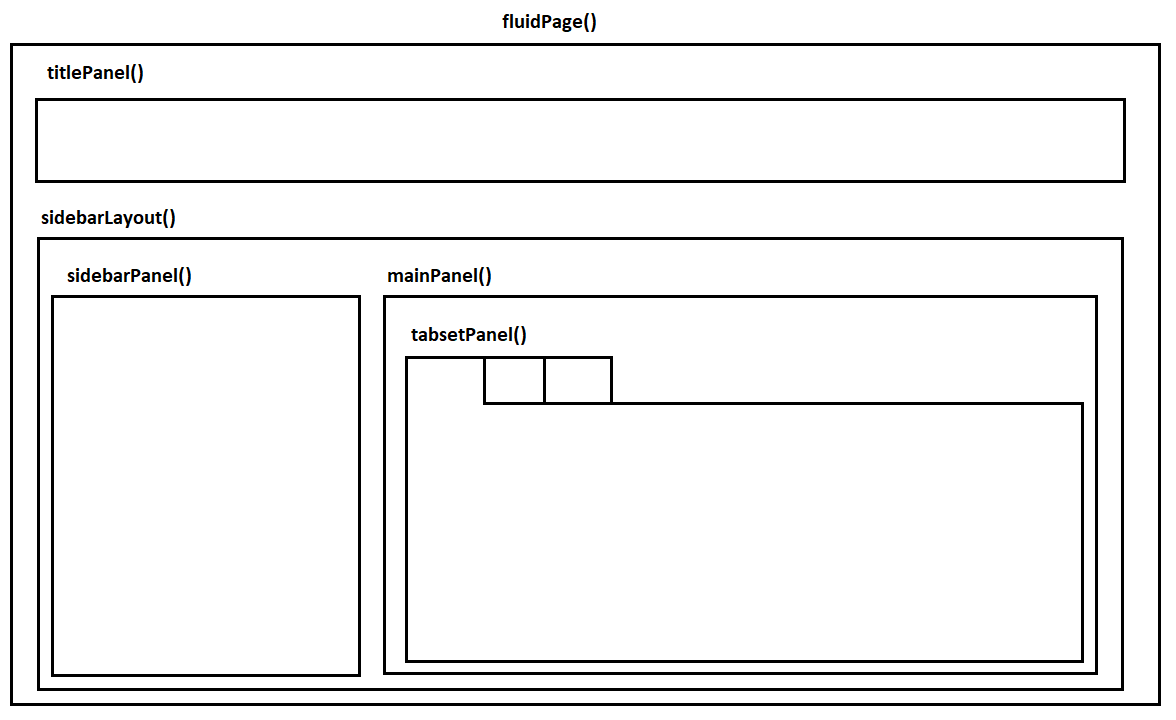
\includegraphics[keepaspectratio]{figures/shinylayout.png}}

The same structure can be represented with code.

\begin{Shaded}
\begin{Highlighting}[]
\NormalTok{ui }\OtherTok{\textless{}{-}} \FunctionTok{fluidPage}\NormalTok{(}
  \FunctionTok{titlePanel}\NormalTok{(}\StringTok{"Title Panel"}\NormalTok{),}
  
  \FunctionTok{sidebarLayout}\NormalTok{(}
    \FunctionTok{sidebarPanel}\NormalTok{(}
      \StringTok{"Side Panel"}
\NormalTok{    ),}
    
    \FunctionTok{mainPanel}\NormalTok{(}
      \StringTok{"Main Panel"}\NormalTok{,}
      
      \FunctionTok{tabsetPanel}\NormalTok{(}
        \FunctionTok{tabPanel}\NormalTok{(}\StringTok{"Tab Panel A"}\NormalTok{),}
        \FunctionTok{tabPanel}\NormalTok{(}\StringTok{"Tab Panel B"}\NormalTok{)}
\NormalTok{      )}
\NormalTok{    )}
\NormalTok{  )}
\NormalTok{)}
\end{Highlighting}
\end{Shaded}

In this chapter we will use a simple sidebar layout without tabs. For a
larger research dashboard, tabs are useful when the app contains
different sections, such as an overview page, a country profile page, a
methods page, and a data table.

\pandocbounded{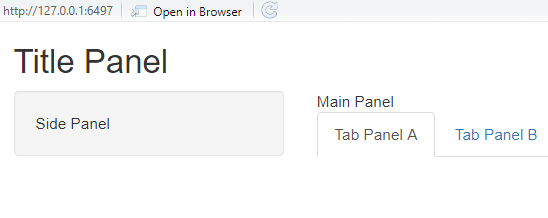
\includegraphics[keepaspectratio]{figures/example_layout.png}}

\section{Adding inputs}\label{adding-inputs}

Inputs collect information from the user.

In this app, we want users to choose a species, choose an island, and
decide whether to show a trend line in the plot.

The first input is a drop-down menu created with \texttt{selectInput()}.

\begin{Shaded}
\begin{Highlighting}[]
\FunctionTok{selectInput}\NormalTok{(}
  \AttributeTok{inputId =} \StringTok{"species"}\NormalTok{,}
  \AttributeTok{label =} \StringTok{"Choose species"}\NormalTok{,}
  \AttributeTok{choices =} \FunctionTok{c}\NormalTok{(}\StringTok{"All"}\NormalTok{, }\FunctionTok{levels}\NormalTok{(penguins}\SpecialCharTok{$}\NormalTok{species)),}
  \AttributeTok{selected =} \StringTok{"All"}
\NormalTok{)}
\end{Highlighting}
\end{Shaded}

The \texttt{inputId} is important. It is the name that the server will
use to read the user selection. If the user chooses \texttt{"Adelie"},
then the server can access that value through \texttt{input\$species}.

The \texttt{label} is the text shown to the user.

The \texttt{choices} are the options available in the menu.

The \texttt{selected} value is the default option.

We use the same structure for island.

\begin{Shaded}
\begin{Highlighting}[]
\FunctionTok{selectInput}\NormalTok{(}
  \AttributeTok{inputId =} \StringTok{"island"}\NormalTok{,}
  \AttributeTok{label =} \StringTok{"Choose island"}\NormalTok{,}
  \AttributeTok{choices =} \FunctionTok{c}\NormalTok{(}\StringTok{"All"}\NormalTok{, }\FunctionTok{levels}\NormalTok{(penguins}\SpecialCharTok{$}\NormalTok{island)),}
  \AttributeTok{selected =} \StringTok{"All"}
\NormalTok{)}
\end{Highlighting}
\end{Shaded}

Finally, we add a checkbox for the trend line.

\begin{Shaded}
\begin{Highlighting}[]
\FunctionTok{checkboxInput}\NormalTok{(}
  \AttributeTok{inputId =} \StringTok{"show\_smooth"}\NormalTok{,}
  \AttributeTok{label =} \StringTok{"Show trend line"}\NormalTok{,}
  \AttributeTok{value =} \ConstantTok{TRUE}
\NormalTok{)}
\end{Highlighting}
\end{Shaded}

A checkbox returns either \texttt{TRUE} or \texttt{FALSE}. In the
server, we will use this value to decide whether to add
\texttt{geom\_smooth()} to the plot.

Now we can place all three inputs inside the sidebar.

\begin{Shaded}
\begin{Highlighting}[]
\NormalTok{ui }\OtherTok{\textless{}{-}} \FunctionTok{fluidPage}\NormalTok{(}
  \FunctionTok{titlePanel}\NormalTok{(}\StringTok{"Palmer Penguins Shiny Demo"}\NormalTok{),}
  
  \FunctionTok{sidebarLayout}\NormalTok{(}
    \FunctionTok{sidebarPanel}\NormalTok{(}
      \FunctionTok{selectInput}\NormalTok{(}
        \AttributeTok{inputId =} \StringTok{"species"}\NormalTok{,}
        \AttributeTok{label =} \StringTok{"Choose species"}\NormalTok{,}
        \AttributeTok{choices =} \FunctionTok{c}\NormalTok{(}\StringTok{"All"}\NormalTok{, }\FunctionTok{levels}\NormalTok{(penguins}\SpecialCharTok{$}\NormalTok{species)),}
        \AttributeTok{selected =} \StringTok{"All"}
\NormalTok{      ),}
      
      \FunctionTok{selectInput}\NormalTok{(}
        \AttributeTok{inputId =} \StringTok{"island"}\NormalTok{,}
        \AttributeTok{label =} \StringTok{"Choose island"}\NormalTok{,}
        \AttributeTok{choices =} \FunctionTok{c}\NormalTok{(}\StringTok{"All"}\NormalTok{, }\FunctionTok{levels}\NormalTok{(penguins}\SpecialCharTok{$}\NormalTok{island)),}
        \AttributeTok{selected =} \StringTok{"All"}
\NormalTok{      ),}
      
      \FunctionTok{checkboxInput}\NormalTok{(}
        \AttributeTok{inputId =} \StringTok{"show\_smooth"}\NormalTok{,}
        \AttributeTok{label =} \StringTok{"Show trend line"}\NormalTok{,}
        \AttributeTok{value =} \ConstantTok{TRUE}
\NormalTok{      )}
\NormalTok{    ),}
    
    \FunctionTok{mainPanel}\NormalTok{(}
      \StringTok{"Outputs will go here"}
\NormalTok{    )}
\NormalTok{  )}
\NormalTok{)}
\end{Highlighting}
\end{Shaded}

At this point, the app has controls, but they do not affect anything
yet. Inputs only become useful when the server uses them.

\section{Adding outputs}\label{adding-outputs}

Outputs define what appears in the app.

For this example, we want three outputs.

We want a printed summary.

\begin{Shaded}
\begin{Highlighting}[]
\FunctionTok{verbatimTextOutput}\NormalTok{(}\StringTok{"summary\_text"}\NormalTok{)}
\end{Highlighting}
\end{Shaded}

We want a plot.

\begin{Shaded}
\begin{Highlighting}[]
\FunctionTok{plotOutput}\NormalTok{(}\StringTok{"penguin\_plot"}\NormalTok{, }\AttributeTok{height =} \StringTok{"450px"}\NormalTok{)}
\end{Highlighting}
\end{Shaded}

And we want an interactive table.

\begin{Shaded}
\begin{Highlighting}[]
\FunctionTok{DTOutput}\NormalTok{(}\StringTok{"penguin\_table"}\NormalTok{)}
\end{Highlighting}
\end{Shaded}

The names inside these functions are output IDs. They must match objects
created in the server.

For example, if the UI contains this output,

\begin{Shaded}
\begin{Highlighting}[]
\FunctionTok{plotOutput}\NormalTok{(}\StringTok{"penguin\_plot"}\NormalTok{)}
\end{Highlighting}
\end{Shaded}

then the server must create this object.

\begin{Shaded}
\begin{Highlighting}[]
\NormalTok{output}\SpecialCharTok{$}\NormalTok{penguin\_plot }\OtherTok{\textless{}{-}} \FunctionTok{renderPlot}\NormalTok{(\{}
  \CommentTok{\# plot code goes here}
\NormalTok{\})}
\end{Highlighting}
\end{Shaded}

This is one of the most important rules in \texttt{Shiny}.

The UI places an output on the page. The server creates the content for
that output. The names must match.

Now we can add the outputs to the main panel.

\begin{Shaded}
\begin{Highlighting}[]
\NormalTok{ui }\OtherTok{\textless{}{-}} \FunctionTok{fluidPage}\NormalTok{(}
  \FunctionTok{titlePanel}\NormalTok{(}\StringTok{"Palmer Penguins Shiny Demo"}\NormalTok{),}
  
  \FunctionTok{sidebarLayout}\NormalTok{(}
    \FunctionTok{sidebarPanel}\NormalTok{(}
      \FunctionTok{selectInput}\NormalTok{(}
        \AttributeTok{inputId =} \StringTok{"species"}\NormalTok{,}
        \AttributeTok{label =} \StringTok{"Choose species"}\NormalTok{,}
        \AttributeTok{choices =} \FunctionTok{c}\NormalTok{(}\StringTok{"All"}\NormalTok{, }\FunctionTok{levels}\NormalTok{(penguins}\SpecialCharTok{$}\NormalTok{species)),}
        \AttributeTok{selected =} \StringTok{"All"}
\NormalTok{      ),}
      
      \FunctionTok{selectInput}\NormalTok{(}
        \AttributeTok{inputId =} \StringTok{"island"}\NormalTok{,}
        \AttributeTok{label =} \StringTok{"Choose island"}\NormalTok{,}
        \AttributeTok{choices =} \FunctionTok{c}\NormalTok{(}\StringTok{"All"}\NormalTok{, }\FunctionTok{levels}\NormalTok{(penguins}\SpecialCharTok{$}\NormalTok{island)),}
        \AttributeTok{selected =} \StringTok{"All"}
\NormalTok{      ),}
      
      \FunctionTok{checkboxInput}\NormalTok{(}
        \AttributeTok{inputId =} \StringTok{"show\_smooth"}\NormalTok{,}
        \AttributeTok{label =} \StringTok{"Show trend line"}\NormalTok{,}
        \AttributeTok{value =} \ConstantTok{TRUE}
\NormalTok{      )}
\NormalTok{    ),}
    
    \FunctionTok{mainPanel}\NormalTok{(}
      \FunctionTok{h3}\NormalTok{(}\StringTok{"Summary"}\NormalTok{),}
      \FunctionTok{verbatimTextOutput}\NormalTok{(}\StringTok{"summary\_text"}\NormalTok{),}
      
      \FunctionTok{h3}\NormalTok{(}\StringTok{"Scatterplot"}\NormalTok{),}
      \FunctionTok{plotOutput}\NormalTok{(}\StringTok{"penguin\_plot"}\NormalTok{, }\AttributeTok{height =} \StringTok{"450px"}\NormalTok{),}
      
      \FunctionTok{h3}\NormalTok{(}\StringTok{"Data"}\NormalTok{),}
      \FunctionTok{DTOutput}\NormalTok{(}\StringTok{"penguin\_table"}\NormalTok{)}
\NormalTok{    )}
\NormalTok{  )}
\NormalTok{)}
\end{Highlighting}
\end{Shaded}

The user interface is now ready. It tells the app what the user sees,
but it still does not tell R how to produce the outputs.

That happens in the server.

\section{Building the server}\label{building-the-server}

The server is where the app does the work.

Every server function has this structure.

\begin{Shaded}
\begin{Highlighting}[]
\NormalTok{server }\OtherTok{\textless{}{-}} \ControlFlowTok{function}\NormalTok{(input, output) \{}
  
\NormalTok{\}}
\end{Highlighting}
\end{Shaded}

The \texttt{input} object contains values selected by the user. The
\texttt{output} object contains the results sent back to the interface.

For example, if the UI contains an input called \texttt{"species"}, then
the server can read the selected species with \texttt{input\$species}.

If the UI contains an output called \texttt{"summary\_text"}, then the
server can create it with \texttt{output\$summary\_text}.

The server code for a printed summary looks like this.

\begin{Shaded}
\begin{Highlighting}[]
\NormalTok{server }\OtherTok{\textless{}{-}} \ControlFlowTok{function}\NormalTok{(input, output) \{}
  
\NormalTok{  output}\SpecialCharTok{$}\NormalTok{summary\_text }\OtherTok{\textless{}{-}} \FunctionTok{renderPrint}\NormalTok{(\{}
\NormalTok{    data }\OtherTok{\textless{}{-}}\NormalTok{ penguins}
    
    \ControlFlowTok{if}\NormalTok{ (input}\SpecialCharTok{$}\NormalTok{species }\SpecialCharTok{!=} \StringTok{"All"}\NormalTok{) \{}
\NormalTok{      data }\OtherTok{\textless{}{-}}\NormalTok{ data }\SpecialCharTok{|\textgreater{}}
        \FunctionTok{filter}\NormalTok{(species }\SpecialCharTok{==}\NormalTok{ input}\SpecialCharTok{$}\NormalTok{species)}
\NormalTok{    \}}
    
    \ControlFlowTok{if}\NormalTok{ (input}\SpecialCharTok{$}\NormalTok{island }\SpecialCharTok{!=} \StringTok{"All"}\NormalTok{) \{}
\NormalTok{      data }\OtherTok{\textless{}{-}}\NormalTok{ data }\SpecialCharTok{|\textgreater{}}
        \FunctionTok{filter}\NormalTok{(island }\SpecialCharTok{==}\NormalTok{ input}\SpecialCharTok{$}\NormalTok{island)}
\NormalTok{    \}}
    
    \FunctionTok{cat}\NormalTok{(}\StringTok{"Rows:"}\NormalTok{, }\FunctionTok{nrow}\NormalTok{(data), }\StringTok{"}\SpecialCharTok{\textbackslash{}n}\StringTok{"}\NormalTok{)}
    \FunctionTok{cat}\NormalTok{(}\StringTok{"Species:"}\NormalTok{, }\FunctionTok{paste}\NormalTok{(}\FunctionTok{unique}\NormalTok{(data}\SpecialCharTok{$}\NormalTok{species), }\AttributeTok{collapse =} \StringTok{", "}\NormalTok{), }\StringTok{"}\SpecialCharTok{\textbackslash{}n}\StringTok{"}\NormalTok{)}
    \FunctionTok{cat}\NormalTok{(}\StringTok{"Islands:"}\NormalTok{, }\FunctionTok{paste}\NormalTok{(}\FunctionTok{unique}\NormalTok{(data}\SpecialCharTok{$}\NormalTok{island), }\AttributeTok{collapse =} \StringTok{", "}\NormalTok{), }\StringTok{"}\SpecialCharTok{\textbackslash{}n}\StringTok{"}\NormalTok{)}
    \FunctionTok{cat}\NormalTok{(}
      \StringTok{"Average body mass:"}\NormalTok{,}
      \FunctionTok{round}\NormalTok{(}\FunctionTok{mean}\NormalTok{(data}\SpecialCharTok{$}\NormalTok{body\_mass\_g, }\AttributeTok{na.rm =} \ConstantTok{TRUE}\NormalTok{), }\DecValTok{1}\NormalTok{),}
      \StringTok{"g}\SpecialCharTok{\textbackslash{}n}\StringTok{"}
\NormalTok{    )}
\NormalTok{  \})}
\NormalTok{\}}
\end{Highlighting}
\end{Shaded}

This code creates an output called \texttt{summary\_text}.

The UI displays that output with
\texttt{verbatimTextOutput("summary\_text")}.

Inside \texttt{renderPrint()}, we first copy the full penguins data into
an object called \texttt{data}. Then we filter it depending on the user
selections. If the selected species is not \texttt{"All"}, we keep only
the selected species. If the selected island is not \texttt{"All"}, we
keep only the selected island.

Finally, we print a few summary lines using \texttt{cat()}.

This is reactive because the code depends on \texttt{input\$species} and
\texttt{input\$island}. When either input changes, Shiny reruns the code
inside \texttt{renderPrint()} and updates the summary.

\section{Adding the plot}\label{adding-the-plot}

The plot works in the same way.

The UI contains this output.

\begin{Shaded}
\begin{Highlighting}[]
\FunctionTok{plotOutput}\NormalTok{(}\StringTok{"penguin\_plot"}\NormalTok{, }\AttributeTok{height =} \StringTok{"450px"}\NormalTok{)}
\end{Highlighting}
\end{Shaded}

The server creates it with \texttt{renderPlot()}.

\begin{Shaded}
\begin{Highlighting}[]
\NormalTok{output}\SpecialCharTok{$}\NormalTok{penguin\_plot }\OtherTok{\textless{}{-}} \FunctionTok{renderPlot}\NormalTok{(\{}
\NormalTok{  data }\OtherTok{\textless{}{-}}\NormalTok{ penguins}
  
  \ControlFlowTok{if}\NormalTok{ (input}\SpecialCharTok{$}\NormalTok{species }\SpecialCharTok{!=} \StringTok{"All"}\NormalTok{) \{}
\NormalTok{    data }\OtherTok{\textless{}{-}}\NormalTok{ data }\SpecialCharTok{|\textgreater{}}
      \FunctionTok{filter}\NormalTok{(species }\SpecialCharTok{==}\NormalTok{ input}\SpecialCharTok{$}\NormalTok{species)}
\NormalTok{  \}}
  
  \ControlFlowTok{if}\NormalTok{ (input}\SpecialCharTok{$}\NormalTok{island }\SpecialCharTok{!=} \StringTok{"All"}\NormalTok{) \{}
\NormalTok{    data }\OtherTok{\textless{}{-}}\NormalTok{ data }\SpecialCharTok{|\textgreater{}}
      \FunctionTok{filter}\NormalTok{(island }\SpecialCharTok{==}\NormalTok{ input}\SpecialCharTok{$}\NormalTok{island)}
\NormalTok{  \}}
  
\NormalTok{  data }\OtherTok{\textless{}{-}}\NormalTok{ data }\SpecialCharTok{|\textgreater{}}
    \FunctionTok{filter}\NormalTok{(}
      \SpecialCharTok{!}\FunctionTok{is.na}\NormalTok{(flipper\_length\_mm),}
      \SpecialCharTok{!}\FunctionTok{is.na}\NormalTok{(body\_mass\_g)}
\NormalTok{    )}
  
\NormalTok{  p }\OtherTok{\textless{}{-}} \FunctionTok{ggplot}\NormalTok{(}
\NormalTok{    data,}
    \FunctionTok{aes}\NormalTok{(}
      \AttributeTok{x =}\NormalTok{ flipper\_length\_mm,}
      \AttributeTok{y =}\NormalTok{ body\_mass\_g,}
      \AttributeTok{colour =}\NormalTok{ species}
\NormalTok{    )}
\NormalTok{  ) }\SpecialCharTok{+}
    \FunctionTok{geom\_point}\NormalTok{(}\AttributeTok{size =} \DecValTok{3}\NormalTok{, }\AttributeTok{alpha =} \FloatTok{0.8}\NormalTok{) }\SpecialCharTok{+}
    \FunctionTok{labs}\NormalTok{(}
      \AttributeTok{x =} \StringTok{"Flipper length, mm"}\NormalTok{,}
      \AttributeTok{y =} \StringTok{"Body mass, g"}\NormalTok{,}
      \AttributeTok{colour =} \StringTok{"Species"}\NormalTok{,}
      \AttributeTok{title =} \StringTok{"Body mass and flipper length"}
\NormalTok{    ) }\SpecialCharTok{+}
    \FunctionTok{theme\_minimal}\NormalTok{(}\AttributeTok{base\_size =} \DecValTok{14}\NormalTok{)}
  
  \ControlFlowTok{if}\NormalTok{ (input}\SpecialCharTok{$}\NormalTok{show\_smooth) \{}
\NormalTok{    p }\OtherTok{\textless{}{-}}\NormalTok{ p }\SpecialCharTok{+} \FunctionTok{geom\_smooth}\NormalTok{(}\AttributeTok{method =} \StringTok{"lm"}\NormalTok{, }\AttributeTok{se =} \ConstantTok{FALSE}\NormalTok{)}
\NormalTok{  \}}
  
\NormalTok{  p}
\NormalTok{\})}
\end{Highlighting}
\end{Shaded}

The first part of the code filters the data. The second part creates the
plot. The final \texttt{if} statement checks whether the user selected
the trend line option. If \texttt{input\$show\_smooth} is \texttt{TRUE},
the app adds a linear trend line.

This is a basic example of conditional display. The plot changes
depending on what the user asks to see.

In a research dashboard, the same logic might control whether to display
confidence intervals, labels, countries in a region, model
specifications, or alternative indicators.

\section{Adding the table}\label{adding-the-table}

The table output is created with \texttt{DT}.

The UI contains this output.

\begin{Shaded}
\begin{Highlighting}[]
\FunctionTok{DTOutput}\NormalTok{(}\StringTok{"penguin\_table"}\NormalTok{)}
\end{Highlighting}
\end{Shaded}

The server creates it with \texttt{renderDT()}.

\begin{Shaded}
\begin{Highlighting}[]
\NormalTok{output}\SpecialCharTok{$}\NormalTok{penguin\_table }\OtherTok{\textless{}{-}} \FunctionTok{renderDT}\NormalTok{(\{}
\NormalTok{  data }\OtherTok{\textless{}{-}}\NormalTok{ penguins}
  
  \ControlFlowTok{if}\NormalTok{ (input}\SpecialCharTok{$}\NormalTok{species }\SpecialCharTok{!=} \StringTok{"All"}\NormalTok{) \{}
\NormalTok{    data }\OtherTok{\textless{}{-}}\NormalTok{ data }\SpecialCharTok{|\textgreater{}}
      \FunctionTok{filter}\NormalTok{(species }\SpecialCharTok{==}\NormalTok{ input}\SpecialCharTok{$}\NormalTok{species)}
\NormalTok{  \}}
  
  \ControlFlowTok{if}\NormalTok{ (input}\SpecialCharTok{$}\NormalTok{island }\SpecialCharTok{!=} \StringTok{"All"}\NormalTok{) \{}
\NormalTok{    data }\OtherTok{\textless{}{-}}\NormalTok{ data }\SpecialCharTok{|\textgreater{}}
      \FunctionTok{filter}\NormalTok{(island }\SpecialCharTok{==}\NormalTok{ input}\SpecialCharTok{$}\NormalTok{island)}
\NormalTok{  \}}
  
  \FunctionTok{datatable}\NormalTok{(}
\NormalTok{    data,}
    \AttributeTok{options =} \FunctionTok{list}\NormalTok{(}\AttributeTok{pageLength =} \DecValTok{8}\NormalTok{),}
    \AttributeTok{rownames =} \ConstantTok{FALSE}
\NormalTok{  )}
\NormalTok{\})}
\end{Highlighting}
\end{Shaded}

This gives the user an interactive table with search and pagination. For
research dashboards, tables are often just as important as plots. They
let users inspect the actual observations behind a visualization.

This is especially useful when the dashboard presents case
classifications, coding decisions, country indicators, or project
metadata.

\section{Avoiding repeated filtering}\label{avoiding-repeated-filtering}

The current app repeats the same filtering code three times. The
summary, plot, and table all begin by creating a filtered version of the
data.

This works, but it is not ideal.

A cleaner approach is to create one reactive object that stores the
filtered data. Then each output can reuse that same object.

In Shiny, this is done with \texttt{reactive()}.

\begin{Shaded}
\begin{Highlighting}[]
\NormalTok{filtered\_penguins }\OtherTok{\textless{}{-}} \FunctionTok{reactive}\NormalTok{(\{}
\NormalTok{  data }\OtherTok{\textless{}{-}}\NormalTok{ penguins}
  
  \ControlFlowTok{if}\NormalTok{ (input}\SpecialCharTok{$}\NormalTok{species }\SpecialCharTok{!=} \StringTok{"All"}\NormalTok{) \{}
\NormalTok{    data }\OtherTok{\textless{}{-}}\NormalTok{ data }\SpecialCharTok{|\textgreater{}}
      \FunctionTok{filter}\NormalTok{(species }\SpecialCharTok{==}\NormalTok{ input}\SpecialCharTok{$}\NormalTok{species)}
\NormalTok{  \}}
  
  \ControlFlowTok{if}\NormalTok{ (input}\SpecialCharTok{$}\NormalTok{island }\SpecialCharTok{!=} \StringTok{"All"}\NormalTok{) \{}
\NormalTok{    data }\OtherTok{\textless{}{-}}\NormalTok{ data }\SpecialCharTok{|\textgreater{}}
      \FunctionTok{filter}\NormalTok{(island }\SpecialCharTok{==}\NormalTok{ input}\SpecialCharTok{$}\NormalTok{island)}
\NormalTok{  \}}
  
\NormalTok{  data}
\NormalTok{\})}
\end{Highlighting}
\end{Shaded}

A reactive object is like a small function. To use it, we call it with
parentheses.

\begin{Shaded}
\begin{Highlighting}[]
\NormalTok{data }\OtherTok{\textless{}{-}} \FunctionTok{filtered\_penguins}\NormalTok{()}
\end{Highlighting}
\end{Shaded}

This lets us simplify the server.

\begin{Shaded}
\begin{Highlighting}[]
\NormalTok{server }\OtherTok{\textless{}{-}} \ControlFlowTok{function}\NormalTok{(input, output) \{}
  
\NormalTok{  filtered\_penguins }\OtherTok{\textless{}{-}} \FunctionTok{reactive}\NormalTok{(\{}
\NormalTok{    data }\OtherTok{\textless{}{-}}\NormalTok{ penguins}
    
    \ControlFlowTok{if}\NormalTok{ (input}\SpecialCharTok{$}\NormalTok{species }\SpecialCharTok{!=} \StringTok{"All"}\NormalTok{) \{}
\NormalTok{      data }\OtherTok{\textless{}{-}}\NormalTok{ data }\SpecialCharTok{|\textgreater{}}
        \FunctionTok{filter}\NormalTok{(species }\SpecialCharTok{==}\NormalTok{ input}\SpecialCharTok{$}\NormalTok{species)}
\NormalTok{    \}}
    
    \ControlFlowTok{if}\NormalTok{ (input}\SpecialCharTok{$}\NormalTok{island }\SpecialCharTok{!=} \StringTok{"All"}\NormalTok{) \{}
\NormalTok{      data }\OtherTok{\textless{}{-}}\NormalTok{ data }\SpecialCharTok{|\textgreater{}}
        \FunctionTok{filter}\NormalTok{(island }\SpecialCharTok{==}\NormalTok{ input}\SpecialCharTok{$}\NormalTok{island)}
\NormalTok{    \}}
    
\NormalTok{    data}
\NormalTok{  \})}
  
\NormalTok{  output}\SpecialCharTok{$}\NormalTok{summary\_text }\OtherTok{\textless{}{-}} \FunctionTok{renderPrint}\NormalTok{(\{}
\NormalTok{    data }\OtherTok{\textless{}{-}} \FunctionTok{filtered\_penguins}\NormalTok{()}
    
    \FunctionTok{cat}\NormalTok{(}\StringTok{"Rows:"}\NormalTok{, }\FunctionTok{nrow}\NormalTok{(data), }\StringTok{"}\SpecialCharTok{\textbackslash{}n}\StringTok{"}\NormalTok{)}
    \FunctionTok{cat}\NormalTok{(}\StringTok{"Species:"}\NormalTok{, }\FunctionTok{paste}\NormalTok{(}\FunctionTok{unique}\NormalTok{(data}\SpecialCharTok{$}\NormalTok{species), }\AttributeTok{collapse =} \StringTok{", "}\NormalTok{), }\StringTok{"}\SpecialCharTok{\textbackslash{}n}\StringTok{"}\NormalTok{)}
    \FunctionTok{cat}\NormalTok{(}\StringTok{"Islands:"}\NormalTok{, }\FunctionTok{paste}\NormalTok{(}\FunctionTok{unique}\NormalTok{(data}\SpecialCharTok{$}\NormalTok{island), }\AttributeTok{collapse =} \StringTok{", "}\NormalTok{), }\StringTok{"}\SpecialCharTok{\textbackslash{}n}\StringTok{"}\NormalTok{)}
    \FunctionTok{cat}\NormalTok{(}
      \StringTok{"Average body mass:"}\NormalTok{,}
      \FunctionTok{round}\NormalTok{(}\FunctionTok{mean}\NormalTok{(data}\SpecialCharTok{$}\NormalTok{body\_mass\_g, }\AttributeTok{na.rm =} \ConstantTok{TRUE}\NormalTok{), }\DecValTok{1}\NormalTok{),}
      \StringTok{"g}\SpecialCharTok{\textbackslash{}n}\StringTok{"}
\NormalTok{    )}
\NormalTok{  \})}
  
\NormalTok{  output}\SpecialCharTok{$}\NormalTok{penguin\_plot }\OtherTok{\textless{}{-}} \FunctionTok{renderPlot}\NormalTok{(\{}
\NormalTok{    data }\OtherTok{\textless{}{-}} \FunctionTok{filtered\_penguins}\NormalTok{() }\SpecialCharTok{|\textgreater{}}
      \FunctionTok{filter}\NormalTok{(}
        \SpecialCharTok{!}\FunctionTok{is.na}\NormalTok{(flipper\_length\_mm),}
        \SpecialCharTok{!}\FunctionTok{is.na}\NormalTok{(body\_mass\_g)}
\NormalTok{      )}
    
\NormalTok{    p }\OtherTok{\textless{}{-}} \FunctionTok{ggplot}\NormalTok{(}
\NormalTok{      data,}
      \FunctionTok{aes}\NormalTok{(}
        \AttributeTok{x =}\NormalTok{ flipper\_length\_mm,}
        \AttributeTok{y =}\NormalTok{ body\_mass\_g,}
        \AttributeTok{colour =}\NormalTok{ species}
\NormalTok{      )}
\NormalTok{    ) }\SpecialCharTok{+}
      \FunctionTok{geom\_point}\NormalTok{(}\AttributeTok{size =} \DecValTok{3}\NormalTok{, }\AttributeTok{alpha =} \FloatTok{0.8}\NormalTok{) }\SpecialCharTok{+}
      \FunctionTok{labs}\NormalTok{(}
        \AttributeTok{x =} \StringTok{"Flipper length, mm"}\NormalTok{,}
        \AttributeTok{y =} \StringTok{"Body mass, g"}\NormalTok{,}
        \AttributeTok{colour =} \StringTok{"Species"}\NormalTok{,}
        \AttributeTok{title =} \StringTok{"Body mass and flipper length"}
\NormalTok{      ) }\SpecialCharTok{+}
      \FunctionTok{theme\_minimal}\NormalTok{(}\AttributeTok{base\_size =} \DecValTok{14}\NormalTok{)}
    
    \ControlFlowTok{if}\NormalTok{ (input}\SpecialCharTok{$}\NormalTok{show\_smooth) \{}
\NormalTok{      p }\OtherTok{\textless{}{-}}\NormalTok{ p }\SpecialCharTok{+} \FunctionTok{geom\_smooth}\NormalTok{(}\AttributeTok{method =} \StringTok{"lm"}\NormalTok{, }\AttributeTok{se =} \ConstantTok{FALSE}\NormalTok{)}
\NormalTok{    \}}
    
\NormalTok{    p}
\NormalTok{  \})}
  
\NormalTok{  output}\SpecialCharTok{$}\NormalTok{penguin\_table }\OtherTok{\textless{}{-}} \FunctionTok{renderDT}\NormalTok{(\{}
    \FunctionTok{datatable}\NormalTok{(}
      \FunctionTok{filtered\_penguins}\NormalTok{(),}
      \AttributeTok{options =} \FunctionTok{list}\NormalTok{(}\AttributeTok{pageLength =} \DecValTok{8}\NormalTok{),}
      \AttributeTok{rownames =} \ConstantTok{FALSE}
\NormalTok{    )}
\NormalTok{  \})}
\NormalTok{\}}
\end{Highlighting}
\end{Shaded}

This is closer to how a real dashboard should be written. If we later
change the filtering logic, we only need to change it once.

\section{The complete app}\label{the-complete-app}

Here is the complete version of the app.

Save this file as \texttt{app.R}.

\begin{Shaded}
\begin{Highlighting}[]
\CommentTok{\# File Name: app.R}
\CommentTok{\# Simple Palmer Penguins Shiny App}

\CommentTok{\# Set up {-}{-}{-}{-}{-}{-}{-}{-}{-}{-}{-}{-}{-}{-}{-}{-}{-}{-}{-}{-}{-}{-}{-}{-}{-}{-}{-}{-}{-}{-}{-}{-}{-}{-}{-}{-}{-}{-}{-}{-}{-}{-}{-}{-}{-}{-}{-}{-}{-}{-}{-}{-}{-}{-}{-}{-}{-}{-}{-}{-}{-}{-}{-}{-}{-}{-}{-}{-}{-}{-}}

\FunctionTok{library}\NormalTok{(shiny)}
\FunctionTok{library}\NormalTok{(palmerpenguins)}
\FunctionTok{library}\NormalTok{(dplyr)}
\FunctionTok{library}\NormalTok{(ggplot2)}
\FunctionTok{library}\NormalTok{(DT)}

\CommentTok{\# Data {-}{-}{-}{-}{-}{-}{-}{-}{-}{-}{-}{-}{-}{-}{-}{-}{-}{-}{-}{-}{-}{-}{-}{-}{-}{-}{-}{-}{-}{-}{-}{-}{-}{-}{-}{-}{-}{-}{-}{-}{-}{-}{-}{-}{-}{-}{-}{-}{-}{-}{-}{-}{-}{-}{-}{-}{-}{-}{-}{-}{-}{-}{-}{-}{-}{-}{-}{-}{-}{-}{-}{-}}

\NormalTok{penguins }\OtherTok{\textless{}{-}}\NormalTok{ palmerpenguins}\SpecialCharTok{::}\NormalTok{penguins }\SpecialCharTok{|\textgreater{}}
  \FunctionTok{mutate}\NormalTok{(}
    \AttributeTok{species =} \FunctionTok{as.factor}\NormalTok{(species),}
    \AttributeTok{island =} \FunctionTok{as.factor}\NormalTok{(island)}
\NormalTok{  )}

\CommentTok{\# User interface {-}{-}{-}{-}{-}{-}{-}{-}{-}{-}{-}{-}{-}{-}{-}{-}{-}{-}{-}{-}{-}{-}{-}{-}{-}{-}{-}{-}{-}{-}{-}{-}{-}{-}{-}{-}{-}{-}{-}{-}{-}{-}{-}{-}{-}{-}{-}{-}{-}{-}{-}{-}{-}{-}{-}{-}{-}{-}{-}{-}{-}{-}}

\NormalTok{ui }\OtherTok{\textless{}{-}} \FunctionTok{fluidPage}\NormalTok{(}
  \FunctionTok{titlePanel}\NormalTok{(}\StringTok{"Palmer Penguins Shiny Demo"}\NormalTok{),}
  
  \FunctionTok{sidebarLayout}\NormalTok{(}
    \FunctionTok{sidebarPanel}\NormalTok{(}
      \FunctionTok{selectInput}\NormalTok{(}
        \AttributeTok{inputId =} \StringTok{"species"}\NormalTok{,}
        \AttributeTok{label =} \StringTok{"Choose species"}\NormalTok{,}
        \AttributeTok{choices =} \FunctionTok{c}\NormalTok{(}\StringTok{"All"}\NormalTok{, }\FunctionTok{levels}\NormalTok{(penguins}\SpecialCharTok{$}\NormalTok{species)),}
        \AttributeTok{selected =} \StringTok{"All"}
\NormalTok{      ),}
      
      \FunctionTok{selectInput}\NormalTok{(}
        \AttributeTok{inputId =} \StringTok{"island"}\NormalTok{,}
        \AttributeTok{label =} \StringTok{"Choose island"}\NormalTok{,}
        \AttributeTok{choices =} \FunctionTok{c}\NormalTok{(}\StringTok{"All"}\NormalTok{, }\FunctionTok{levels}\NormalTok{(penguins}\SpecialCharTok{$}\NormalTok{island)),}
        \AttributeTok{selected =} \StringTok{"All"}
\NormalTok{      ),}
      
      \FunctionTok{checkboxInput}\NormalTok{(}
        \AttributeTok{inputId =} \StringTok{"show\_smooth"}\NormalTok{,}
        \AttributeTok{label =} \StringTok{"Show trend line"}\NormalTok{,}
        \AttributeTok{value =} \ConstantTok{TRUE}
\NormalTok{      )}
\NormalTok{    ),}
    
    \FunctionTok{mainPanel}\NormalTok{(}
      \FunctionTok{h3}\NormalTok{(}\StringTok{"Summary"}\NormalTok{),}
      \FunctionTok{verbatimTextOutput}\NormalTok{(}\StringTok{"summary\_text"}\NormalTok{),}
      
      \FunctionTok{h3}\NormalTok{(}\StringTok{"Scatterplot"}\NormalTok{),}
      \FunctionTok{plotOutput}\NormalTok{(}\StringTok{"penguin\_plot"}\NormalTok{, }\AttributeTok{height =} \StringTok{"450px"}\NormalTok{),}
      
      \FunctionTok{h3}\NormalTok{(}\StringTok{"Data"}\NormalTok{),}
      \FunctionTok{DTOutput}\NormalTok{(}\StringTok{"penguin\_table"}\NormalTok{)}
\NormalTok{    )}
\NormalTok{  )}
\NormalTok{)}

\CommentTok{\# Server {-}{-}{-}{-}{-}{-}{-}{-}{-}{-}{-}{-}{-}{-}{-}{-}{-}{-}{-}{-}{-}{-}{-}{-}{-}{-}{-}{-}{-}{-}{-}{-}{-}{-}{-}{-}{-}{-}{-}{-}{-}{-}{-}{-}{-}{-}{-}{-}{-}{-}{-}{-}{-}{-}{-}{-}{-}{-}{-}{-}{-}{-}{-}{-}{-}{-}{-}{-}{-}{-}}

\NormalTok{server }\OtherTok{\textless{}{-}} \ControlFlowTok{function}\NormalTok{(input, output) \{}
  
\NormalTok{  filtered\_penguins }\OtherTok{\textless{}{-}} \FunctionTok{reactive}\NormalTok{(\{}
\NormalTok{    data }\OtherTok{\textless{}{-}}\NormalTok{ penguins}
    
    \ControlFlowTok{if}\NormalTok{ (input}\SpecialCharTok{$}\NormalTok{species }\SpecialCharTok{!=} \StringTok{"All"}\NormalTok{) \{}
\NormalTok{      data }\OtherTok{\textless{}{-}}\NormalTok{ data }\SpecialCharTok{|\textgreater{}}
        \FunctionTok{filter}\NormalTok{(species }\SpecialCharTok{==}\NormalTok{ input}\SpecialCharTok{$}\NormalTok{species)}
\NormalTok{    \}}
    
    \ControlFlowTok{if}\NormalTok{ (input}\SpecialCharTok{$}\NormalTok{island }\SpecialCharTok{!=} \StringTok{"All"}\NormalTok{) \{}
\NormalTok{      data }\OtherTok{\textless{}{-}}\NormalTok{ data }\SpecialCharTok{|\textgreater{}}
        \FunctionTok{filter}\NormalTok{(island }\SpecialCharTok{==}\NormalTok{ input}\SpecialCharTok{$}\NormalTok{island)}
\NormalTok{    \}}
    
\NormalTok{    data}
\NormalTok{  \})}
  
\NormalTok{  output}\SpecialCharTok{$}\NormalTok{summary\_text }\OtherTok{\textless{}{-}} \FunctionTok{renderPrint}\NormalTok{(\{}
\NormalTok{    data }\OtherTok{\textless{}{-}} \FunctionTok{filtered\_penguins}\NormalTok{()}
    
    \FunctionTok{cat}\NormalTok{(}\StringTok{"Rows:"}\NormalTok{, }\FunctionTok{nrow}\NormalTok{(data), }\StringTok{"}\SpecialCharTok{\textbackslash{}n}\StringTok{"}\NormalTok{)}
    \FunctionTok{cat}\NormalTok{(}\StringTok{"Species:"}\NormalTok{, }\FunctionTok{paste}\NormalTok{(}\FunctionTok{unique}\NormalTok{(data}\SpecialCharTok{$}\NormalTok{species), }\AttributeTok{collapse =} \StringTok{", "}\NormalTok{), }\StringTok{"}\SpecialCharTok{\textbackslash{}n}\StringTok{"}\NormalTok{)}
    \FunctionTok{cat}\NormalTok{(}\StringTok{"Islands:"}\NormalTok{, }\FunctionTok{paste}\NormalTok{(}\FunctionTok{unique}\NormalTok{(data}\SpecialCharTok{$}\NormalTok{island), }\AttributeTok{collapse =} \StringTok{", "}\NormalTok{), }\StringTok{"}\SpecialCharTok{\textbackslash{}n}\StringTok{"}\NormalTok{)}
    \FunctionTok{cat}\NormalTok{(}
      \StringTok{"Average body mass:"}\NormalTok{,}
      \FunctionTok{round}\NormalTok{(}\FunctionTok{mean}\NormalTok{(data}\SpecialCharTok{$}\NormalTok{body\_mass\_g, }\AttributeTok{na.rm =} \ConstantTok{TRUE}\NormalTok{), }\DecValTok{1}\NormalTok{),}
      \StringTok{"g}\SpecialCharTok{\textbackslash{}n}\StringTok{"}
\NormalTok{    )}
\NormalTok{  \})}
  
\NormalTok{  output}\SpecialCharTok{$}\NormalTok{penguin\_plot }\OtherTok{\textless{}{-}} \FunctionTok{renderPlot}\NormalTok{(\{}
\NormalTok{    data }\OtherTok{\textless{}{-}} \FunctionTok{filtered\_penguins}\NormalTok{() }\SpecialCharTok{|\textgreater{}}
      \FunctionTok{filter}\NormalTok{(}
        \SpecialCharTok{!}\FunctionTok{is.na}\NormalTok{(flipper\_length\_mm),}
        \SpecialCharTok{!}\FunctionTok{is.na}\NormalTok{(body\_mass\_g)}
\NormalTok{      )}
    
\NormalTok{    p }\OtherTok{\textless{}{-}} \FunctionTok{ggplot}\NormalTok{(}
\NormalTok{      data,}
      \FunctionTok{aes}\NormalTok{(}
        \AttributeTok{x =}\NormalTok{ flipper\_length\_mm,}
        \AttributeTok{y =}\NormalTok{ body\_mass\_g,}
        \AttributeTok{colour =}\NormalTok{ species}
\NormalTok{      )}
\NormalTok{    ) }\SpecialCharTok{+}
      \FunctionTok{geom\_point}\NormalTok{(}\AttributeTok{size =} \DecValTok{3}\NormalTok{, }\AttributeTok{alpha =} \FloatTok{0.8}\NormalTok{) }\SpecialCharTok{+}
      \FunctionTok{labs}\NormalTok{(}
        \AttributeTok{x =} \StringTok{"Flipper length, mm"}\NormalTok{,}
        \AttributeTok{y =} \StringTok{"Body mass, g"}\NormalTok{,}
        \AttributeTok{colour =} \StringTok{"Species"}\NormalTok{,}
        \AttributeTok{title =} \StringTok{"Body mass and flipper length"}
\NormalTok{      ) }\SpecialCharTok{+}
      \FunctionTok{theme\_minimal}\NormalTok{(}\AttributeTok{base\_size =} \DecValTok{14}\NormalTok{)}
    
    \ControlFlowTok{if}\NormalTok{ (input}\SpecialCharTok{$}\NormalTok{show\_smooth) \{}
\NormalTok{      p }\OtherTok{\textless{}{-}}\NormalTok{ p }\SpecialCharTok{+} \FunctionTok{geom\_smooth}\NormalTok{(}\AttributeTok{method =} \StringTok{"lm"}\NormalTok{, }\AttributeTok{se =} \ConstantTok{FALSE}\NormalTok{)}
\NormalTok{    \}}
    
\NormalTok{    p}
\NormalTok{  \})}
  
\NormalTok{  output}\SpecialCharTok{$}\NormalTok{penguin\_table }\OtherTok{\textless{}{-}} \FunctionTok{renderDT}\NormalTok{(\{}
    \FunctionTok{datatable}\NormalTok{(}
      \FunctionTok{filtered\_penguins}\NormalTok{(),}
      \AttributeTok{options =} \FunctionTok{list}\NormalTok{(}\AttributeTok{pageLength =} \DecValTok{8}\NormalTok{),}
      \AttributeTok{rownames =} \ConstantTok{FALSE}
\NormalTok{    )}
\NormalTok{  \})}
\NormalTok{\}}

\CommentTok{\# Run app {-}{-}{-}{-}{-}{-}{-}{-}{-}{-}{-}{-}{-}{-}{-}{-}{-}{-}{-}{-}{-}{-}{-}{-}{-}{-}{-}{-}{-}{-}{-}{-}{-}{-}{-}{-}{-}{-}{-}{-}{-}{-}{-}{-}{-}{-}{-}{-}{-}{-}{-}{-}{-}{-}{-}{-}{-}{-}{-}{-}{-}{-}{-}{-}{-}{-}{-}{-}{-}}

\FunctionTok{shinyApp}\NormalTok{(}\AttributeTok{ui =}\NormalTok{ ui, }\AttributeTok{server =}\NormalTok{ server)}
\end{Highlighting}
\end{Shaded}

To run the app, open \texttt{app.R} in RStudio and click \textbf{Run
App}.

You can also run the file from the console.

\begin{Shaded}
\begin{Highlighting}[]
\NormalTok{shiny}\SpecialCharTok{::}\FunctionTok{runApp}\NormalTok{()}
\end{Highlighting}
\end{Shaded}

The app should open in a browser window or in the RStudio viewer.

\section{Publishing the app}\label{publishing-the-app}

A Shiny app runs through R. This means that it cannot be published in
exactly the same way as a static HTML page. The server hosting the app
needs to be able to run R.

The easiest route for small teaching apps is
\href{https://www.shinyapps.io/}{shinyapps.io}.

In RStudio, the deployment process is usually done through the publish
button. After creating an account and connecting it to RStudio, you can
publish the app directly from the app window.

\pandocbounded{\includegraphics[keepaspectratio]{figures/deploy.gif}}

For larger projects, other deployment options may be more appropriate.
These include Posit Connect, a university server, a virtual machine,
Docker, or a cloud service such as Google Cloud Run.

The important point is that a Shiny app is not just a file. It is an
application that needs an R environment.

\section{From teaching example to research
dashboard}\label{from-teaching-example-to-research-dashboard}

The penguins example is deliberately simple, but the structure maps
directly onto research dashboards.

The species filter could become a country filter.

The island filter could become a region, institution, policy area, or
year filter.

The scatterplot could become a trend plot, indicator comparison, model
output, map, or timeline.

The table could become a searchable database of cases, documents,
interviews, coding decisions, or country profiles.

The summary text could become a short country note, a methodological
explanation, or a dynamic description of the selected data.

The important design question is not whether we can make everything
interactive. We usually can. The better question is which forms of
interactivity help the reader understand the research more clearly.

A useful research dashboard should not be a dumping ground for every
object produced during a project. It should give the user controlled
access to selected parts of the evidence base.

\section{A simple research dashboard
structure}\label{a-simple-research-dashboard-structure}

A practical research dashboard often has four sections.

The first section is an overview. It tells the user what the dashboard
contains, what the unit of analysis is, and what the user can do with
it.

The second section is an exploration page. This is where users filter
data, compare cases, and inspect plots.

The third section is a data page. This gives users access to the
underlying table, usually with search and download options.

The fourth section is a methods or documentation page. This explains
where the data come from, how variables were coded, and what limitations
the user should keep in mind.

In Shiny, this can be organized with tabs.

\begin{Shaded}
\begin{Highlighting}[]
\NormalTok{ui }\OtherTok{\textless{}{-}} \FunctionTok{fluidPage}\NormalTok{(}
  \FunctionTok{titlePanel}\NormalTok{(}\StringTok{"Research Dashboard"}\NormalTok{),}
  
  \FunctionTok{tabsetPanel}\NormalTok{(}
    \FunctionTok{tabPanel}\NormalTok{(}
      \StringTok{"Overview"}\NormalTok{,}
      \FunctionTok{h3}\NormalTok{(}\StringTok{"About this dashboard"}\NormalTok{),}
      \FunctionTok{p}\NormalTok{(}\StringTok{"Short project description goes here."}\NormalTok{)}
\NormalTok{    ),}
    
    \FunctionTok{tabPanel}\NormalTok{(}
      \StringTok{"Explore"}\NormalTok{,}
      \FunctionTok{sidebarLayout}\NormalTok{(}
        \FunctionTok{sidebarPanel}\NormalTok{(}
          \FunctionTok{selectInput}\NormalTok{(}
            \AttributeTok{inputId =} \StringTok{"country"}\NormalTok{,}
            \AttributeTok{label =} \StringTok{"Choose country"}\NormalTok{,}
            \AttributeTok{choices =} \FunctionTok{c}\NormalTok{(}\StringTok{"All"}\NormalTok{, }\StringTok{"Country A"}\NormalTok{, }\StringTok{"Country B"}\NormalTok{)}
\NormalTok{          )}
\NormalTok{        ),}
        \FunctionTok{mainPanel}\NormalTok{(}
          \FunctionTok{plotOutput}\NormalTok{(}\StringTok{"main\_plot"}\NormalTok{)}
\NormalTok{        )}
\NormalTok{      )}
\NormalTok{    ),}
    
    \FunctionTok{tabPanel}\NormalTok{(}
      \StringTok{"Data"}\NormalTok{,}
      \FunctionTok{DTOutput}\NormalTok{(}\StringTok{"data\_table"}\NormalTok{)}
\NormalTok{    ),}
    
    \FunctionTok{tabPanel}\NormalTok{(}
      \StringTok{"Methods"}\NormalTok{,}
      \FunctionTok{h3}\NormalTok{(}\StringTok{"Data and coding"}\NormalTok{),}
      \FunctionTok{p}\NormalTok{(}\StringTok{"Documentation goes here."}\NormalTok{)}
\NormalTok{    )}
\NormalTok{  )}
\NormalTok{)}
\end{Highlighting}
\end{Shaded}

This structure is often enough for a first version of a research
dashboard.

\section{Common mistakes}\label{common-mistakes}

The most common mistake is building the interface before deciding what
the dashboard is for. A dashboard should begin with a small number of
user questions. For example, the user may want to compare countries,
inspect a time trend, check the coding of a case, or download a filtered
table. The app should be designed around those tasks.

A second mistake is making everything reactive. Interactivity is useful
only when it changes something meaningful. Too many controls make the
app harder to read.

A third mistake is hiding the data. Research dashboards should usually
include a table or documentation page. This helps users understand what
they are seeing and reduces the risk that the dashboard becomes a
decorative object.

A fourth mistake is forgetting that the app needs to be maintained. If
the data are updated manually, the dashboard should make that clear. If
the app depends on external files, APIs, or packages, those dependencies
should be documented.

\section{Conclusion}\label{conclusion-1}

The basic structure of a Shiny dashboard is simple. The UI defines what
the user sees. The server defines what R calculates. Inputs collect
information from the user. Render functions create outputs. Reactive
objects help the app update when inputs change.

Once this structure is clear, larger dashboards become less mysterious.
They may have more files, more data, more tabs, and better design, but
they still follow the same logic.

For research communication, the value of a dashboard is not that it
looks impressive. The value is that it lets users inspect a project in a
controlled and transparent way. A good dashboard makes it easier to see
what the data contain, how cases compare, and what choices sit behind
the final outputs.

\bookmarksetup{startatroot}

\chapter*{References}\label{references}
\addcontentsline{toc}{chapter}{References}

\markboth{References}{References}

\phantomsection\label{refs}
\begin{CSLReferences}{1}{0}
\bibitem[\citeproctext]{ref-chang2018}
Chang, Winston. 2018. \emph{R Graphics Cookbook: Practical Recipes for
Visualizing Data}. Second. Sebastopol, California: O'Reilly Media.
\url{https://r-graphics.org/}.

\bibitem[\citeproctext]{ref-lovelace2016}
Gillespie, Colin, and Robin Lovelace. 2016. \emph{Efficient r
Programming: A Practical Guide to Smarter Programming}. Sebastopol,
California: O'Reilly Media.
\url{https://csgillespie.github.io/efficientR/}.

\bibitem[\citeproctext]{ref-grolemund2014}
Grolemund, Garrett. 2014. \emph{Hands-on Programming with r: Write Your
Own Functions and Simulations}. Sebastopol, California: O'Reilly Media.
\url{https://rstudio-education.github.io/hopr/}.

\bibitem[\citeproctext]{ref-wickham2016}
Grolemund, Garrett, and Hadley Wickham. 2016. \emph{R for Data Science}.
Sebastopol, California: O'Reilly Media. \url{https://r4ds.had.co.nz/}.

\bibitem[\citeproctext]{ref-long2019}
Long, JD, and Paul Teetor. 2019. \emph{R Cookbook: Proven Recipes for
Data Analysis, Statistics, and Graphics}. Second. Sebastopol,
California: O'Reilly Media. \url{https://rc2e.com/}.

\bibitem[\citeproctext]{ref-mcmanus2014}
Mcmanus, Ian, and Paul Gesiak. 2014. {``Experimenting with Mondrian:
Comparing the Method of Production with the Method of Choice.''} In.
\url{https://doi.org/10.13140/2.1.1561.2967}.

\bibitem[\citeproctext]{ref-silge2017}
Silge, Julia, and David Robinson. 2017. \emph{Text Mining with r: A Tidy
Approach}. Sebastopol, California: O'Reilly Media.
\url{https://www.tidytextmining.com/}.

\bibitem[\citeproctext]{ref-venables21}
Venables, W. N., D. M. Smith, and the R Core Team. 2021. \emph{An
Introduction to r}.
\url{https://cran.r-project.org/doc/manuals/R-intro.pdf}.

\bibitem[\citeproctext]{ref-wilke2019}
Wilke, Claus O. 2019. \emph{Fundamentals of Data Visualization: A Primer
on Making Informative and Compelling Figures}. Sebastopol, California:
O'Reilly Media. \url{https://clauswilke.com/dataviz/}.

\bibitem[\citeproctext]{ref-wilkinson2005}
Wilkinson, Leland. 2005. \emph{The Grammar of Graphics}. 2nd ed. New
York: Springer-Verlag.
\url{https://www.springer.com/gp/book/9780387245447}.

\bibitem[\citeproctext]{ref-xie2018}
Xie, Yihui, J. J. Allaire, and Garrett Grolemund. 2018. \emph{R
Markdown: The Definitive Guide}. Boca Raton, Florida: Chapman; Hall/CRC.
\url{https://bookdown.org/yihui/rmarkdown}.

\bibitem[\citeproctext]{ref-xie2020}
Xie, Yihui, Christophe Dervieux, and Emily Riederer. 2020. \emph{R
Markdown Cookbook}. Boca Raton, Florida: Chapman; Hall/CRC.
\url{https://bookdown.org/yihui/rmarkdown-cookbook}.

\bibitem[\citeproctext]{ref-zinovyev2010}
Zinovyev, iAndrei. 2010. {``Data Visualization in Political and Social
Sciences.''} In. \url{https://arxiv.org/abs/1008.1188}.

\end{CSLReferences}




\end{document}
